%\documentclass{beamer}
%\documentclass[slidestop,usepdftitle=false]{beamer}
\documentclass[english,10pt,table]{beamer}
%\documentclass[english,10pt,table,handout]{beamer}


% Copyright 2007 by Till Tantau
%
% This file may be distributed and/or modified
%
% 1. under the LaTeX Project Public License and/or
% 2. under the GNU Public License.
%
% See the file doc/licenses/LICENSE for more details.


% Common packages

\usepackage[english]{babel}
\usepackage[utf8]{vietnam}
%\usepackage{times}
\usefonttheme[onlymath]{serif}
\usecolortheme{default}
\usepackage{booktabs}
\usepackage{mathpartir}
\usepackage{listings}
\usepackage{pbox}
\mprset{flushleft}
\mode<article>
{
  \usepackage{times}
  \usepackage{mathptmx}
  \usepackage[left=1.5cm,right=6cm,top=1.5cm,bottom=3cm]{geometry}
}

\usepackage{hyperref}
\usepackage{tikz}
\usetikzlibrary{arrows,backgrounds}
%\tikzstyle{mnode}=[circle, draw, fill=black, inner sep=0pt, minimum width=4pt]
\usepackage{colortbl}
%\usepackage{yfonts}
\usepackage{translator} % comment this, if not available


% Common settings for all lectures in this course

\def\lecturename{Báo cáo bài tập lớn}

\title{\insertlecture}

\author{L04-Nhóm 9}

\institute
{
\begin{table}[]
\begin{tabular}{lll}
\multicolumn{1}{c}{} & \multicolumn{1}{c}{} & \multicolumn{1}{c}{}\\
\small{2114066} & \small{Phan Lê Nhật Minh} & \small{minh.phanpvd@hcmut.edu.vn} \\
\small{2110030} & \small{Dương Ngọc Ân} & \small{an.duong110103@hcmut.edu.vn}  \\
\small{2112185} & \small{Cù Hoàng Nguyễn Sơn} & \small{son.cu3856@hcmut.edu.vn}      \\
\small{2112887} & \small{Từ Huy Bảo} & \small{bao.tu4545@hcmut.edu.vn}      \\
\small{2112122} & \small{Nguyễn Hồng Quân} & \small{quan.nguyenhg12@hcmut.edu.vn} \\
\small{2110300} & \small{Lê Văn Tuấn Kiệt} & \small{kiet.le0303@hcmut.edu.vn}     
\end{tabular}
\end{table}
}

\subject{Lecturer \lecturename}




% Beamer version theme settings

\useoutertheme[height=0pt,width=2cm,right]{sidebar}
\usecolortheme{rose,sidebartab}
\useinnertheme{circles}
\usefonttheme[only large]{structurebold}

\setbeamercolor{sidebar right}{bg=black!15}
\setbeamercolor{structure}{fg=blue}
\setbeamercolor{author}{parent=structure}

\setbeamerfont{title}{series=\normalfont,size=\LARGE}
\setbeamerfont{title in sidebar}{series=\bfseries}
\setbeamerfont{author in sidebar}{series=\bfseries}
\setbeamerfont*{item}{series=}
\setbeamerfont{frametitle}{size=}
\setbeamerfont{block title}{size=\small}
\setbeamerfont{subtitle}{size=\normalsize,series=\normalfont}

\setbeamertemplate{navigation symbols}{}
\setbeamertemplate{bibliography item}[book]
\setbeamertemplate{sidebar right}
{
  {\usebeamerfont{title in sidebar}%
    \vskip1.5em%
    \hskip3pt%
    \usebeamercolor[fg]{title in sidebar}%
    \insertshorttitle[width=2cm,center,respectlinebreaks]\par%
    \vskip1.25em%
  }%
  {%
    \hskip3pt%
    \usebeamercolor[fg]{author in sidebar}%
    \usebeamerfont{author in sidebar}%
    \insertshortauthor[width=2cm,center,respectlinebreaks]\par%
    \vskip1.25em%
  }%
  \hbox to2cm{\hss\insertlogo\hss}
  \vskip1.25em%
  \insertverticalnavigation{2cm}%
  \vfill
  \hbox to 2cm{\hfill\usebeamerfont{subsection in
      sidebar}\strut\usebeamercolor[fg]{subsection in
      sidebar}\insertshortlecture.\insertframenumber\hskip5pt}%
  \vskip3pt%
}%

\setbeamertemplate{title page}
{
  \vbox{}
  \vskip1em
  {\huge Chapter \insertshortlecture\par}
  {\usebeamercolor[fg]{title}\usebeamerfont{title}\inserttitle\par}%
  \ifx\insertsubtitle\@empty%
  \else%
    \vskip0.25em%
    {\usebeamerfont{subtitle}\usebeamercolor[fg]{subtitle}\insertsubtitle\par}%
  \fi%     
  \vskip1em\par
  \emph{\lecturename}\ on \insertdate\par
  \vskip0pt plus1filll
  \leftskip=0pt plus1fill\insertauthor\par
  \insertinstitute\vskip1em
}

\logo{
\includegraphics[width=1.5cm]{hcmut.png}}



% Article version layout settings

\mode<article>

\makeatletter
\def\@listI{\leftmargin\leftmargini
  \parsep 0pt
  \topsep 5\p@   \@plus3\p@ \@minus5\p@
  \itemsep0pt}
\let\@listi=\@listI


\setbeamertemplate{frametitle}{\paragraph*{\insertframetitle\
    \ \small\insertframesubtitle}\ \par
}
\setbeamertemplate{frame end}{%
  \marginpar{\scriptsize\hbox to 1cm{\sffamily%
      \hfill\strut\insertshortlecture.\insertframenumber}\hrule height .2pt}}
\setlength{\marginparwidth}{1cm}
\setlength{\marginparsep}{4.5cm}

\def\@maketitle{\makechapter}

\def\makechapter{
  \newpage
  \null
  \vskip 2em%
  {%
    \parindent=0pt
    \raggedright
    \sffamily
    \vskip8pt
    {\fontsize{36pt}{36pt}\selectfont Chapter \insertshortlecture \par\vskip2pt}
    {\fontsize{24pt}{28pt}\selectfont \color{blue!50!black} \insertlecture\par\vskip4pt}
    {\Large\selectfont \color{blue!50!black} \insertsubtitle\par}
    \vskip10pt

    \normalsize\selectfont Print version of
    Lecturer \emph{\lecturename} of \@date\par\vskip1.5em
    \hfill Tran Vinh Tan, Faculty of CSE, University of Technology
  }
  \par
  \vskip 1.5em%
}

\let\origstartsection=\@startsection
\def\@startsection#1#2#3#4#5#6{%
  \origstartsection{#1}{#2}{#3}{#4}{#5}{#6\normalfont\sffamily\color{blue!50!black}\selectfont}}

\makeatother

\mode
<all>




% Typesetting Listings

\usepackage{listings}
\lstset{language=Java}

\alt<presentation>
{\lstset{%
  basicstyle=\footnotesize\ttfamily,
  commentstyle=\slshape\color{green!50!black},
  keywordstyle=\bfseries\color{blue!50!black},
  identifierstyle=\color{blue},
  stringstyle=\color{orange},
  escapechar=\#,
  emphstyle=\color{red}}
}
{
  \lstset{%
    basicstyle=\ttfamily,
    keywordstyle=\bfseries,
    commentstyle=\itshape,
    escapechar=\#,
    emphstyle=\bfseries\color{red}
  }
}



% Common theorem-like environments

\theoremstyle{example}
\newtheorem{exercise}[theorem]{\translate{Exercise}}


% New useful definitions:

\newbox\mytempbox
\newdimen\mytempdimen

\newcommand\includegraphicscopyright[3][]{%
  \leavevmode\vbox{\vskip3pt\raggedright\setbox\mytempbox=\hbox{\includegraphics[#1]{#2}}%
    \mytempdimen=\wd\mytempbox\box\mytempbox\par\vskip1pt%
    \fontsize{3}{3.5}\selectfont{\color{black!25}{\vbox{\hsize=\mytempdimen#3}}}\vskip3pt%
}}

\newenvironment{colortabular}[1]{\medskip\rowcolors[]{1}{blue!20}{blue!10}\tabular{#1}\rowcolor{blue!40}}{\endtabular\medskip}

\def\equad{\leavevmode\hbox{}\quad}

\newenvironment{greencolortabular}[1]
{\medskip\rowcolors[]{1}{green!50!black!20}{green!50!black!10}%
  \tabular{#1}\rowcolor{green!50!black!40}}%
{\endtabular\medskip}




\lecture[]{CẤU TRÚC RỜI RẠC CHO KHMT}{}

\usepackage{pifont}
% Symbol definitions for these lists
\newcommand{\DingListSymbolA}{43}
\newcommand{\DingListSymbolB}{243}
\newcommand{\DingListSymbolC}{224}
\newcommand{\DingListSymbolD}{219}

% Boxed equation
\definecolor{LightYellow}{rgb}{1.,1.,.9}
\definecolor{LightRed}{rgb}{1.,.6,.6}


%%ensembles de nombres
\def\NP{$\mathcal{NP}$}
\def\N{\mathbb{N}}
\def\Z{\mathbb{Z}}
\def\R{\mathbb{R}}
\def\Q{\mathbb{Q}}

%\date[]{~~}
%%%%%%%%%%%%%%%%%%%%%%%%%%%%%%%%%%%%%%%%%%%%%%%%%%%%%%%%%%%%%%%%%%%%%
%%%%%%%%%%%%%%%%%%%%%%%%%%%%%%%%%%%%%%%%%%%%%%%%%%%%%%%%%%%%%%%%%%%%%
\begin{document}
\frame{
\selectlanguage{english}
  \maketitle
}


%%%%%%%%%%%%%%%%%%%%%%%%%%%%%%%%%%%%%%%%%%%%%%%%%%%%%%%%%%%%%%%%%%%%%
%%%%%%%%%%%%%%%%%%%%%%%%%%%%%%%%%%%%%%%%%%%%%%%%%%%%%%%%%%%%%%%%%%%%%
%\section[Plan]{}
%\setcounter{tocdepth}{1}
\frame{ \tableofcontents}
%\setcounter{tocdepth}{5}
% to display left summary deeper and plan slide juste display section: add command \setcounter{tocdepth}{1} and then \setcounter{tocdepth}{10}  recompile twice or more again 

%%%%%%%%%%%%%%%%%%%%%%%%%%%%%%%%%%%%%%%%%%%%%%%%%%%%%%%%%%%%%%%%%%%%%
%%%%%%%%%%%%%%%%%%%%%%%%%%%%%%%%%%%%%%%%%%%%%%%%%%%%%%%%%%%%%%%%%%%%%
\section{Động cơ nghiên cứu}
\frame
{
  \frametitle{Động cơ nghiên cứu}	
\begin{block}{Nghiên cứu để làm gì?}
	$\indent$COVID-19 đã tạo ra những tác động tiêu cực đến đời sống của cư dân trên thế giới. Các đợt bùng phát của COVID-19 hay những biến thể virus đã mang đến những thách thức chưa từng có và được dự báo sẽ có tác động đáng kể đến sự phát triển kinh tế.
	Phân tích \& thống kê dữ liệu về COVID-19 giúp cho ta thấy được số ca nhiễm bệnh, tử vong của một quốc gia, so sánh tình trạng của các quốc gia trong khu vực hay diễn biến dịch trên thế giới. Từ số liệu được báo cáo mới chúng ta muốn biết các ca nhiễm bệnh có xu hướng tăng lên hay giảm xuống quy mô các đợt bùng phát ở mỗi quốc gia.
\end{block}
}

\section{Mục tiêu}
\frame
{
	\frametitle{Mục tiêu}
	\begin{block}{Cần có mục tiêu thiết thực}
$\indent$Trong bài tập lớn này, chúng ta sẽ bắt đầu với các bài toán thống kê đơn giản từ những dữ liệu được cung cấp. Qua đó, ta tìm ra những con số thú vị, có ý nghĩa đối với các dữ liệu thực tế từ tình hình dịch corona. Những kết quả mà ta tìm ra sẽ là bước khởi đầu cho việc khai phá nguồn dữ liệu của hệ thống sau này, nhằm đạt tới mục tiêu nâng cao kỹ năng lập trình, kỹ năng giải quyết vấn đề cho người học, kỹ năng làm việc nhóm cũng như hướng tới mục tiêu cao hơn là đam mê trong làm việc, học tập và nghiên cứu.
		
	\end{block}
}

\section{Mô tả dữ liệu}
\frame
{
    \frametitle{Mô tả dữ liệu}
    \begin{block}{Dữ liệu gồm các thuộc tính chính  {\bf ``iso\_code, continent, location, date, new\_cases,	new\_deaths''} được lưu trong file \textbf{csv}.}
	\begin{enumerate}
		\item $iso\_code$: Định danh đất nước 
		\item $continent$: Tên châu lục
		\item $location$: Tên quốc gia
		\item $date$: Ngày quan sát với định dạng Month-Day-Year
		\item $new\_cases$: Số trường hợp COVID-19 mới được xác nhận 
		\item $new\_deaths$: Số tử vong mới do COVID-19 
	\end{enumerate}
	\end{block}
}

\section{Nhiệm vụ}
\frame
{
    \frametitle{Task 1}
    \begin{block}{Cơ sở lý thuyết}
    \begin{itemize}
        \item Lưu bảng dữ liệu thô vào biến bigTable
        \item Lưu bảng dữ liệu sau khi lọc bớt các hàng không có châu lục vào biến tableNoNull
        \item Lưu các biến này vào preTask.RData bằng câu lệnh save.image("workspace/preTask.RData") để có thể tái sử dụng
        \item Cài đặt một số packages: readr, ggplot2, stringr, dplyr
        \item Một số hàm quan trọng được dùng trong task 1:str\_sub, unique, write và write.csv, subset, append, tail và head, length, data.frame
        \item Cuối cùng, lưu lại các biến để có thể tái sử dụng bằng save.image
    \end{itemize}
    \end{block}
}
\frame
{
    \frametitle{Task 1-Subtask 1}
    \begin{block}{Tập mẫu thể hiện thu thập dữ liệu vào các năm nào:}
    \begin{itemize}
        \item 2020
        \item 2021
        \item 2022
    \end{itemize}
    \end{block}
}
\frame
{
    \frametitle{Task 1-Subtask 2}
    \begin{block}{Số lượng đất nước và định danh của mỗi đất nước:}
    \begin{figure}[H]
        \centering
        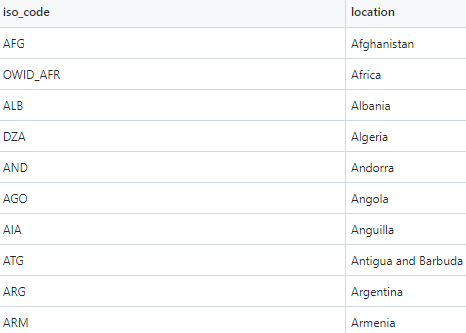
\includegraphics[scale=0.7]{images/1.2.png}
    \end{figure}
    \end{block}
}
\frame
{
    \frametitle{Task 1-Subtask 2}
    \begin{block}{Số lượng đất nước:}
    238
    \end{block}
}
\frame
{
    \frametitle{Task 1-Subtask 3}
    \begin{block}{Số lượng châu lục trong tập mẫu:}
    \begin{figure}
        \centering
        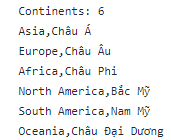
\includegraphics{images/1.3.png}
    \end{figure}
    \end{block}
}
\frame
{
    \frametitle{Task 1-Subtask 4}
    \begin{block}{Số lượng dữ liệu thể hiện thu thập dữ liệu được trong từng châu lục và tổng số:}
    \begin{figure}
        \centering
        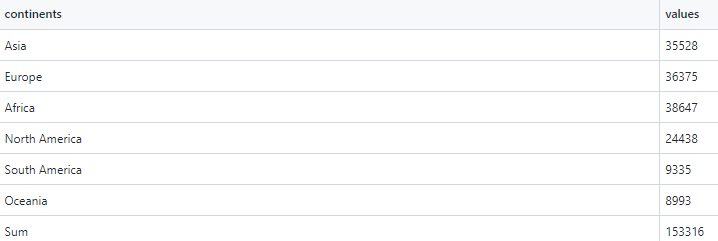
\includegraphics[scale=0.5]{images/1.4.png}
    \end{figure}
    \end{block}
}
\frame
{
    \frametitle{Task 1-Subtask 5}
    \begin{block}{Số lượng dữ liệu thể hiện thu thập dữ liệu được trong từng đất nước (hiển thị 10 dất nước cuối cùng) và tổng s}
    \begin{figure}
        \centering
        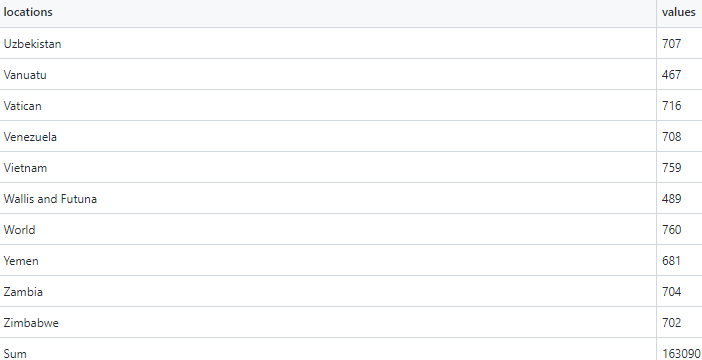
\includegraphics[scale=0.5]{images/1.5.png}
    \end{figure}
    \end{block}
}
\frame
{
    \frametitle{Task 1-Subtask 6}
    \begin{block}{Cho biết các châu lục nào có lượng dữ liệu thu thập nhỏ nhất và giá trị nhỏ nhất đó?}
    Châu lục có lượng dữ liệu thu thập nhỏ nhất là Châu Đại Dương với giá trị là 8993
    \end{block}
}
\frame
{
    \frametitle{Task 1-Subtask 7}
    \begin{block}{Cho biết các châu lục nào có lượng dữ liệu thu thập lớn nhất và giá trị lớn nhất đó?}
    Châu lục có lượng dữ liệu thu thập lớn nhất là Châu Phi với giá trị là 38647
    \end{block}
}
\frame
{
    \frametitle{Task 1-Subtask 8}
    \begin{block}{Cho biết các nước nào có lượng dữ liệu thu thập nhỏ nhất và giá trị nhỏ nhất đó?}
    Nước có ít dữ liệu thu thập nhỏ nhất là Pitcairn với giá trị là 85
    \end{block}
}
\frame
{
    \frametitle{Task 1-Subtask 9}
    \begin{block}{Cho biết các nước nào có lượng dữ liệu thu thập lớn nhất và giá trị lớn nhất đó?}
    Nước có số lượng dữ liệu thu thập lớn nhất là Argentina và Mexico với giá trị là 781
    \end{block}
}
\frame
{
    \frametitle{Task 1-Subtask 10}
    \begin{block}{Cho biết các date nào có lượng dữ liệu thu thập nhỏ nhất và giá trị nhỏ nhất đó?}
    \begin{figure}[H]
				\centering
				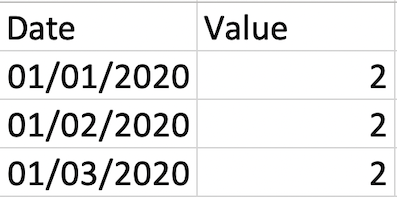
\includegraphics{images/1.10.png}
			\end{figure}
    \end{block}
}
\frame
{
    \frametitle{Task 1-Subtask 11}
    \begin{block}{Cho biết các date nào có lượng dữ liệu thu thập lớn nhất và giá trị lớn nhất đó?}
    \begin{figure}[H]
				\centering
				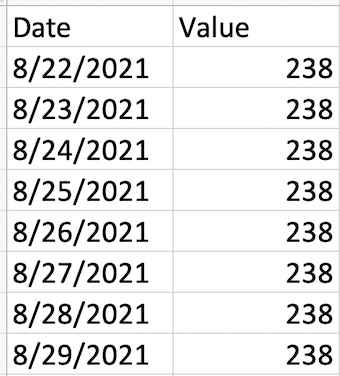
\includegraphics[scale=0.8]{images/1.11.png}
			\end{figure}
    \end{block}
}
\frame
{
    \frametitle{Task 1-Subtask 12}
    \begin{block}{Cho biết số lượng dữ liệu thu thập được theo date và châu lục.}
    \begin{figure}[H]
				\centering
				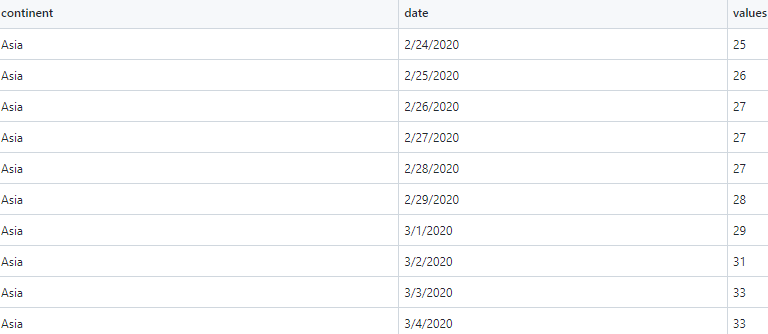
\includegraphics[scale=0.45]{images/1.12.png}
			\end{figure}
    \end{block}
}
\frame
{
    \frametitle{Task 1-Subtask 13}
    \begin{block}{Cho biết số lượng dữ liệu thu thập được là lớn nhất theo date và châu lục}
    \begin{figure}[H]
				\centering
				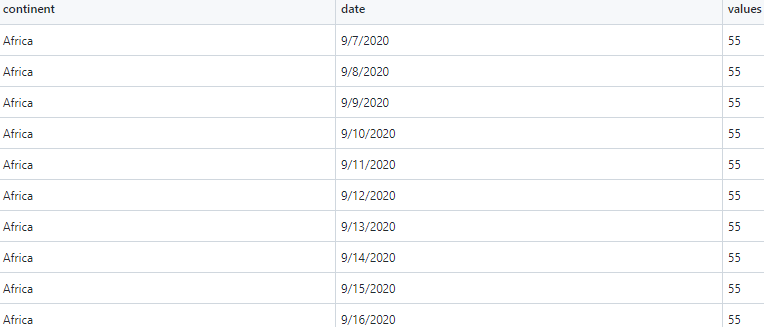
\includegraphics[scale=0.45]{images/1.13.png}
			\end{figure}
    \end{block}
}
\frame
{
    \frametitle{Task 1-Subtask 14}
    \begin{block}{Cho biết số lượng dữ liệu thu thập được là nhỏ nhất theo date và châu lục}
    \begin{figure}[H]
				\centering
				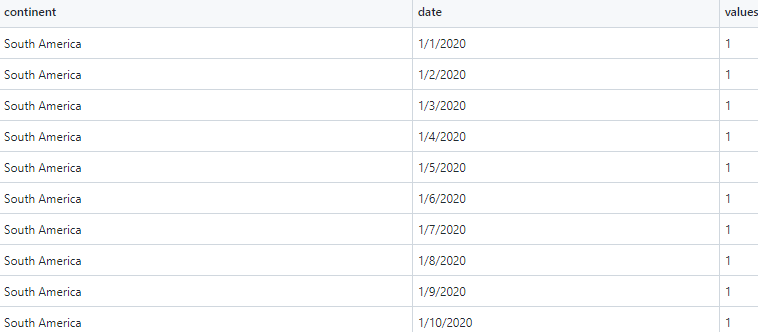
\includegraphics[scale=0.45]{images/1.14.png}
			\end{figure}
    \end{block}
}
\frame
{
    \frametitle{Task 1-Subtask 15}
    \begin{block}{Viết một hàm với một date là k và châu lục t cho trước, cho biết số lượng dữ liệu thể hiện thu thập dữ liệu được}
    \begin{figure}[H]
				\centering
				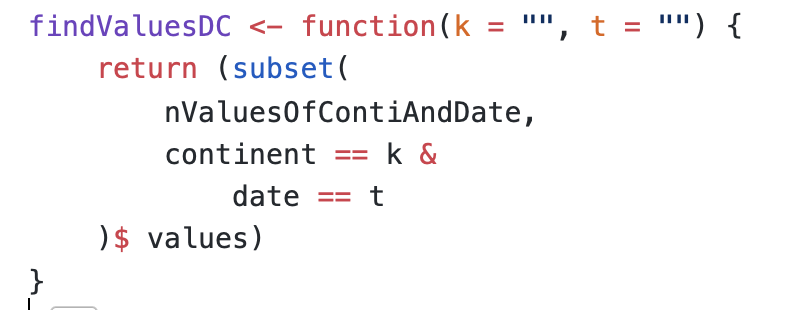
\includegraphics[scale=0.45]{images/1.18.png}
			\end{figure}
    \end{block}
}
\frame
{
    \frametitle{Task 1-Subtask 16}
    \begin{block}{Các đất nước có số lượng dữ liệu thu thập được bằng nhau.}
    \begin{figure}[H]
				\centering
				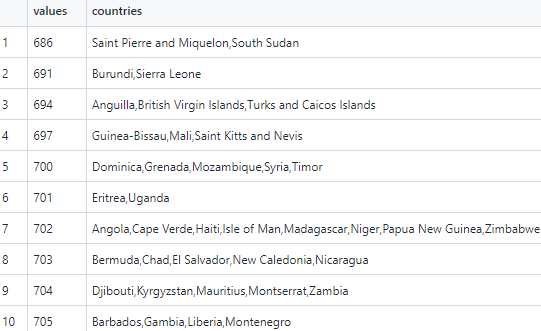
\includegraphics[scale=0.6]{images/1.15.png}
			\end{figure}
    \end{block}
}
\frame
{
    \frametitle{Task 1-Subtask 17}
    \begin{block}{Liệt kê iso\_code, tên đất nước mà chiều dài iso\_code lớn hơn 3}
    \begin{figure}[H]
				\centering
				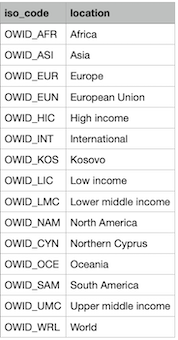
\includegraphics{images/1.17.png}
			\end{figure}
    \end{block}
}
\frame
{
    \frametitle{Task 2}
    \begin{block}{Cơ sở lý thuyết}
    \begin{itemize}
        \item Tứ phân vị là đại lượng mô tả sự phân bố và sự phân tán của tập dữ liệu
        \item Tứ phân vị có 3 giá trị, đó là tứ phân vị thứ nhất, thứ nhì, và thứ ba.
        \item Giá trị tứ phân vị thứ hai Q2 chính bằng giá trị trung vị. Giá trị tứ phân vị thứ nhất Q1 bằng trung vị phần dưới. Giá trị tứ phân vị thứ ba Q3 bằng trung vị phần trên
        \item Trong thống kê mô tả, độ lệch chuẩn là thước đo độ phân tán của một tập hợp các giá trị so với giá trị trung bình của chúng. Độ lệch chuẩn của 1 giá trị càng thấp nghĩa là giá trị đó càng gần với giá trị trung bình của tập hợp.
        \item Biểu đồ hộp (Box plot) là biểu đồ diễn tả 5 vị trí phân bố của dữ liệu, đó là: giá trị nhỏ nhất (min), tứ phân vị thứ nhất (Q1), trung vị (median), tứ phân vị thứ 3 (Q3) và giá trị lớn nhất (max).
        \item Các hàm thường sử dụng trong task 2: names, summary, rownames, colnames, boxplot
    \end{itemize}
    \end{block}
}
\frame
{
    \frametitle{Task 2}
    \begin{block}{Số lượng ca nhiễm mới}
    \begin{figure}
        \centering
        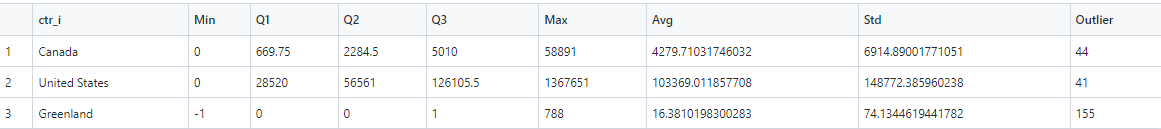
\includegraphics[scale=0.32]{images/2.1.png}
    \end{figure}
    \end{block}
}
\frame
{
    \frametitle{Task 2}
    \begin{block}{Số ca tử vong}
    \begin{figure}
        \centering
        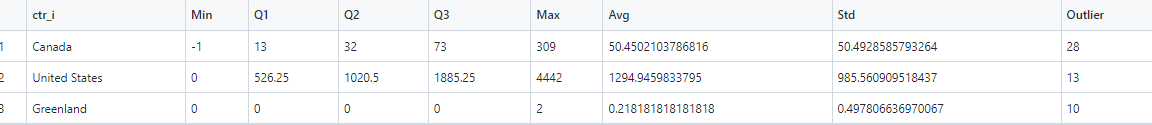
\includegraphics[scale=0.32]{images/2.2.png}
    \end{figure}
    \end{block}
}
\frame
{
    \frametitle{Task 2}
    \begin{block}{Biểu đồ boxplot nhiễm coranavirus}
    \begin{figure}[H]
		\centering
		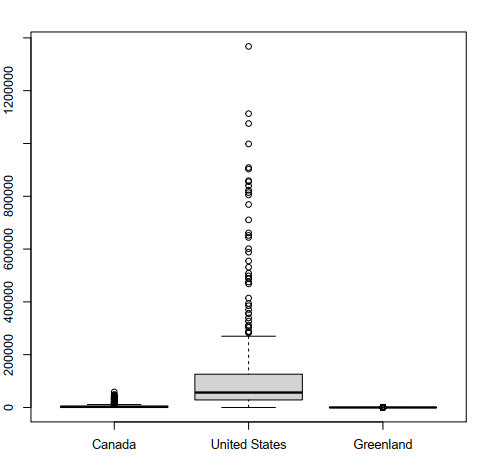
\includegraphics[scale=0.6]{images/2.3.png}
	\end{figure}
    \end{block}
}
\frame
{
    \frametitle{Task 3}
    \begin{block}{Cơ sở lý thuyết}
    $\indent$Sử dụng hàm p\_load của thư viện Pacman ( đã được tích hợp vào R ở phiên bản 4.1.3) để cài các thư viện chưa có sẵn trong máy vào thêm các thư viện vào chương trình
	
	Các thư viện sử dụng:
	    \begin{itemize}
	\item rio: Nhập xuất file
	\item here: Tạo đường dẫn
	\item tibble: Tạo bảng
        \end{itemize}
        \begin{figure}[H]
            \centering
            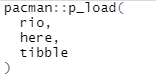
\includegraphics{images/3.0.png}
        \end{figure}
    Nhập file và thiết lập một số giá trị ban đầu
        \begin{itemize}
	\item Sử dụng hàm import kết hợp here để nhập file "owid-covid-data.csv"
	\item Tạo vector “name.country” lưu tên ba nước của nhóm
        \end{itemize}
    \end{block}
}
\frame
{
    \frametitle{Task 3-Subtask 1}
    \begin{block}{Hướng làm}
$\indent$Tạo hàm “ndwithoutrpcases” xử lý yêu cầu đề bài về ca nhiễm khi cung cấp cho hàm tên nước
	    \begin{itemize}
	\item Tạo vector “select” lưu địa chị các dòng chứa tên nước chỉ thị
	\item Sử dụng hàm “subset” với điều kiện là hàm “select” tạo dataframe “covid.data.location” chứa dữ liệu của nước được chọn
	\item Dùng vòng lặp for với số vòng lặp bằng số dòng của của “covid.data.location” đếm số ngày có dữ liệu không được báo cáo mới
	\item Xuất ra giá trị vừa đếm được
	    \begin{figure}[H]
				\centering
				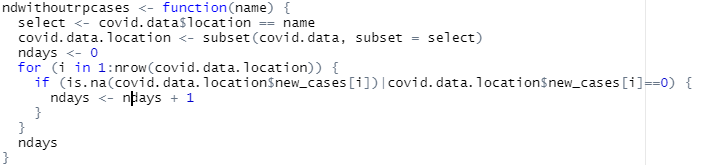
\includegraphics[scale=0.4]{images/3.0.1.png}
		\end{figure}
        \end{itemize}
    \end{block}
}
\frame
{
    \frametitle{Task 3-Subtask 1}
    \begin{block}{Hướng làm}
    $\indent$Sử dụng hàm để tính toán số ngày có dữ liệu ca nhiễm không được báo cáo mới với từng nước, lưu lần lượt giá trị vào 3 biến a, b, c
        \begin{figure}[H]
				\centering
				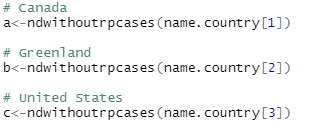
\includegraphics[scale=0.9]{images/3.0.2.png}
		\end{figure}
	$\indent$Xử lý tương tự với ca tử vong, lưu vào ba biến d, e, f
	
	Tạo dataframe “cau1” lưu các giá trị vừa tạo ở trên
        \begin{figure}[H]
				\centering
				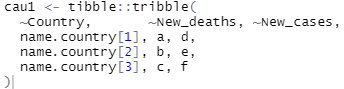
\includegraphics[scale=0.9]{images/3.0.3.png}
		\end{figure}
    \end{block}
}
\frame
{
    \frametitle{Task 3-Subtask 1}
    \begin{block}{Có bao nhiêu ngày có số lần dữ liệu không được báo cáo mới.}
    \begin{figure}[H]
			\centering
			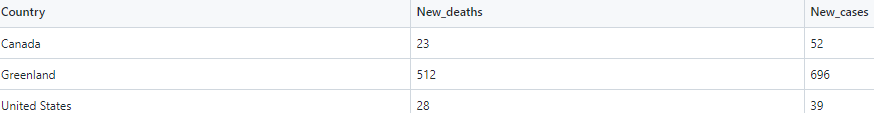
\includegraphics[scale=0.4]{images/3.1.png}
	\end{figure}
    \end{block}
}
\frame
{
    \frametitle{Task 3-Subtask 2}
    \begin{block}{Hướng làm}
        \begin{itemize}
	\item Tạo hàm “nlowestdayscases” để xử lý yêu cầu đề bài về số ca nhiễm khi được cung cấp tên nước
	\item Tạo dataframe “covid.data.location” chứa dữ liệu từng nước tương tự như câu 1
    \item Tạo biến “ndays” và biến “min” để lưu giá trị thấp nhất, thiết lập giá trị ban đầu cho “ndays” và “min” là 0
	\item Sử dụng vòng lặp for kết hợp câu lệnh if ghép để tìm giá trị đầu tiên khác không phải giá trị rỗng và bằng 0, gán giá trị đó là giá trị min đầu tiên
	\item Dùng vòng lặp for đếm số ngày có số ca nhiễm/tử vong là thấp nhất được báo cáo mới
	\item Xuất ra giá trị vừa tìm được
	        \end{itemize}
    \end{block}
}
\frame
{
    \frametitle{Task 3-Subtask 2}
    \begin{block}{Hướng làm}

                \begin{figure}[H]
			\centering
			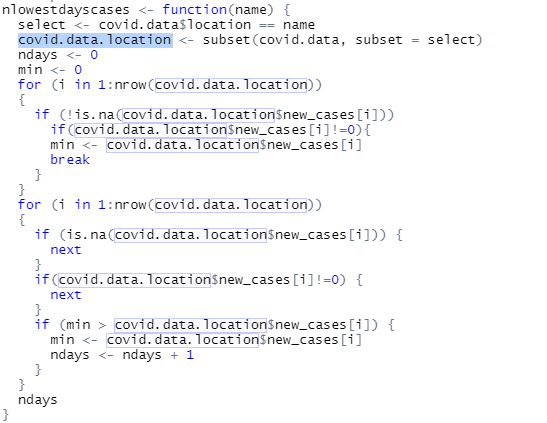
\includegraphics[scale=0.5]{images/3.0.4.png}
		\end{figure}
 Xử lý tương tự ở câu 1, lưu các giá trị lần lượt vào các biến a,b,c,d,e,f sau đó tạo bảng lưu vào dataframe “cau2”

    \end{block}
}
\frame
{
    \frametitle{Task 3-Subtask 2}
    \begin{block}{Có bao nhiêu ngày có số ca nhiễm/ tử vong là thấp nhất được báo cáo mới}
    \begin{figure}[H]
		\centering
		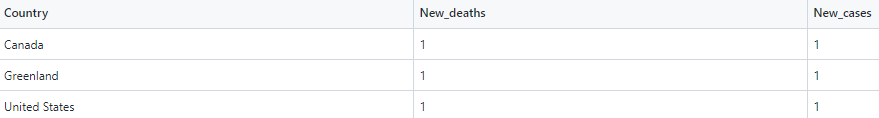
\includegraphics[scale=0.4]{images/3.2.png}
	\end{figure}
    \end{block}
}
\frame
{
    \frametitle{Task 3-Subtask 3}
    \begin{block}{Có bao nhiêu ngày có số ca nhiễm/ tử vong là cao nhất được báo cáo mới}
	\begin{figure}[H]
		\centering
		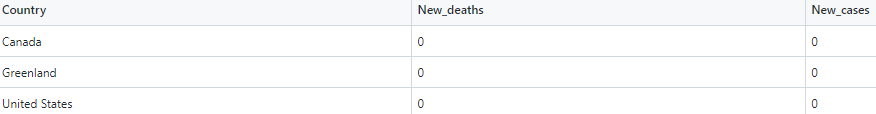
\includegraphics[scale=0.4]{images/3.3.png}
	\end{figure}
    \end{block}
}
\frame
{
    \frametitle{Task 3-Subtask 4}
    \begin{block}{Không được báo cáo mới:}
    \begin{itemize}
	\item Sử dụng hàm subset tạo một dataframe lưu giữ liệu của ba nước về tên nước, số ca nhiễm, số ca tử vong và chỉ giữ lại các hàng có số ca nhiễm hoặc ca tử vong bằng 0 hoặc rỗng
	\item Đổi tên 3 cột thành "Countries", "Infections", "Deaths"
	\item Lưu dataframe vừa tạo vào “cau4a”
			    \end{itemize}
    \begin{figure}[H]
		\centering
		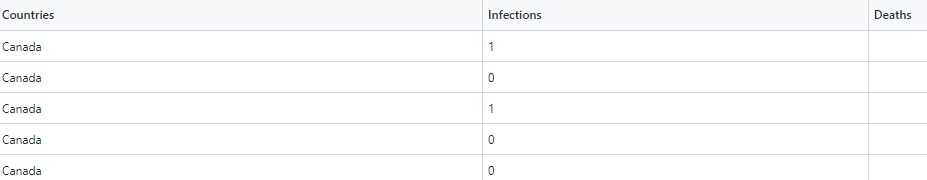
\includegraphics[scale=0.4]{images/3.4.1.png}
		\end{figure}
    \end{block}
}
\frame
{
    \frametitle{Task 3-Subtask 4}
    \begin{block}{Báo cáo mới:}
    \begin{figure}[H]
		\centering
		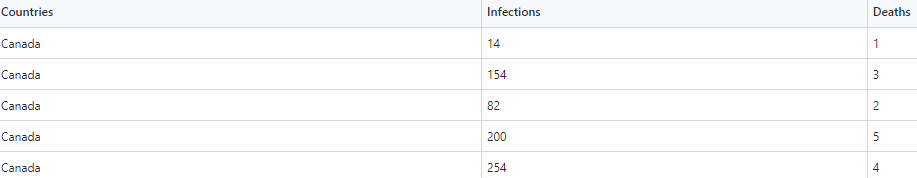
\includegraphics[scale=0.4]{images/3.4.2.png}
	\end{figure}
    \end{block}
}
\frame
{
    \frametitle{Task 3-Subtask 5}
    \begin{block}{Hướng làm}
         \begin{itemize}
	\item Tạo hàm “short.ds.no.report.cases” để xử lý yêu cầu đề bài về số ca nhiễm khi được cung cấp tên nước
	\item Tạo dataframe “covid.data.location” tương tự các câu trước
	\item Tạo biến “inmissing” để xác định có đang ở trong chuỗi ngày không được báo cáo
	\item Tạo biến “length.of.missing” lưu giá trị của số ngày ngắn nhất liên tiếp mà không có dữ liệu được báo cáo, giá trị ban đầu là toàn bộ số ngày có trong dữ liệu
	\item Tạo biến “temp.length” lưu độ dài chuỗi ngày liên tiếp không được báo cáo vòng lặp for đang chỉ vào
	            \begin{figure}[H]
			    	\centering
			    	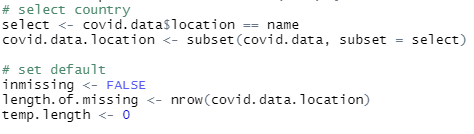
\includegraphics[scale=0.6]{images/3.0.5.png}
		    	\end{figure}
			    \end{itemize}
    \end{block}
}
\frame
{
    \frametitle{Task 3-Subtask 5}
    \begin{block}{Hướng làm}
         \begin{itemize}
	\item Nếu dữ liệu không có ngày nào không được báo cáo dữ liệu, length.of.missing =0
	\item Sử dụng vòng lặp for đếm lần lượt chiều dài của các chuỗi số ngày liên tiếp không được báo cáo dữ liệu lưu vào temp.length, nếu temp.length < length.of.missing, gán giá trị của temp.length cho length.of.missing, lần lượt như vậy cho đến hết chương trình
	\item Trả về kết quả vừa tìm được
	\item Lần lượt xử lí cho các nước và lưu vào các biến a,b,c
	\item Tương tự với ca tử vong và lưu vào các biến d, e, f
	\item Tạo bảng chứa các giá trị vừa tìm và lưu vào “cau5”
			    \end{itemize}
    \end{block}
}
\frame
{
    \frametitle{Task 3-Subtask 5}
    \begin{block}{Cho biết số ngày ngắn nhất liên tiếp mà không có dữ liệu được báo cáo}
    \begin{figure}[H]
		\centering
		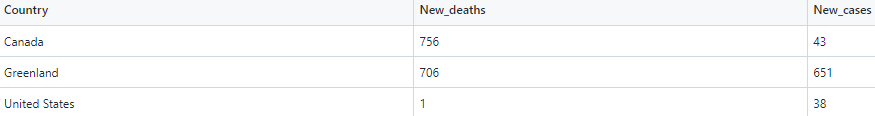
\includegraphics[scale=0.4]{images/3.5.png}
	\end{figure}
    \end{block}
}
\frame
{
    \frametitle{Task 3-Subtask 6}
    \begin{block}{Cho biết số ngày dài nhất liên tiếp mà không có dữ liệu được báo cáo}
    \begin{figure}[H]
		\centering
		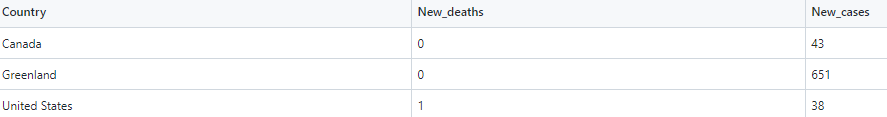
\includegraphics[scale=0.4]{images/3.6.png}
	\end{figure}
    \end{block}
}
\frame
{
    \frametitle{Task 3-Subtask 7}
    \begin{block}{Cho biết số ngày ngắn nhất liên tiếp mà không có người nhiễm bệnh mới}
    \begin{figure}[H]
		\centering
		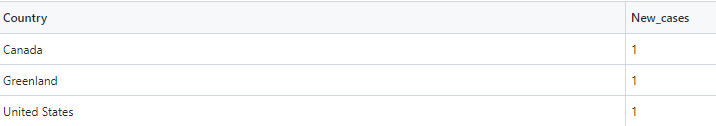
\includegraphics[scale=0.5]{images/3.7.png}
	\end{figure}
    \end{block}
}
\frame
{
    \frametitle{Task 3-Subtask 8}
    \begin{block}{Cho biết số ngày dài nhất liên tiếp mà không có người nhiễm bệnh mới}
    \begin{figure}[H]
		\centering
		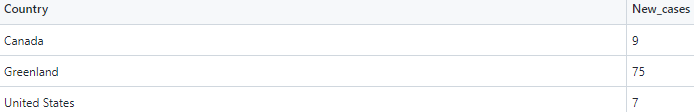
\includegraphics[scale=0.5]{images/3.8.png}
	\end{figure}
    \end{block}
}
\frame
{
    \frametitle{Task 4}
    \begin{block}{Cơ sở lý thuyết}
    \begin{itemize}
        \item Biểu đồ tần số tích lũy (cumulative frequency plots) biểu thị những thông tin dạng tích lũy. Nó thể hiện số lượng hay tỉ lệ những quan sát nhỏ hơn hoặc bằng một giá trị cụ thể
        \item Biểu đồ tần số tương đối cho ta biết lượng dữ liệu mà một quốc gia thu thập chiếm bao nhiêu
phần trăm trong châu lục chứa quốc gia đó.
        \item Biểu đồ phổ thể hiện sự phân phối về số lượng của một tập dữ liệu.
        \item Một số thư viện cần dùng: ggplot2, agricolae, ggpubr, lubridate
        \item Các hàm thường sử dụng trong task 4: ggplot, ggexport, strptime, barplot, hist, max, min, sum
    \end{itemize}
    \end{block}
}
\frame
{
    \frametitle{Task 4-Subtask 1}
    \begin{block}{Biểu đồ tần số tích lũy của Châu Phi}
    \begin{figure}
        \centering
        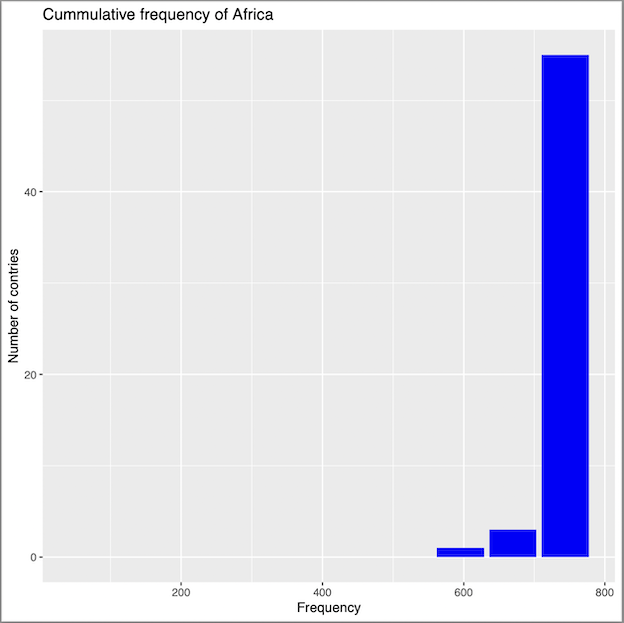
\includegraphics[scale=0.6]{images/4.1.1.png}
    \end{figure}
    \end{block}
}
\frame
{
    \frametitle{Task 4-Subtask 1}
    \begin{block}{Biểu đồ tần số tích lũy của Châu Á}
    \begin{figure}
        \centering
        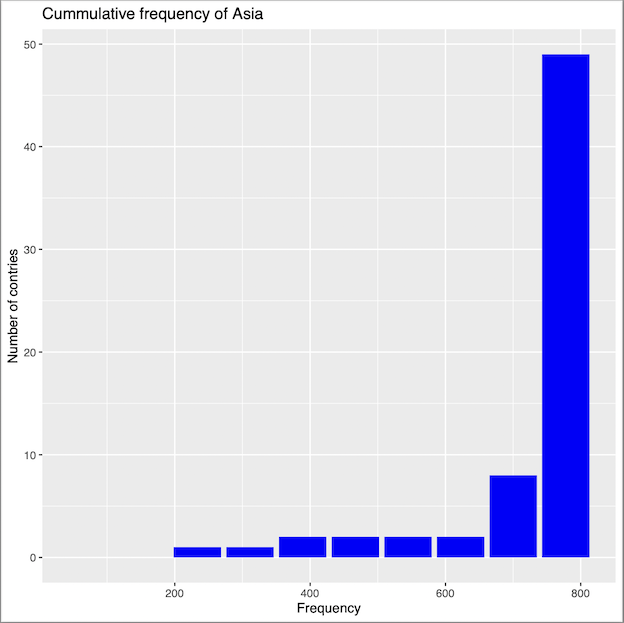
\includegraphics[scale=0.6]{images/4.1.2.png}
    \end{figure}
    \end{block}
}
\frame
{
    \frametitle{Task 4-Subtask 1}
    \begin{block}{Biểu đồ tần số tích lũy của Châu Âu}
    \begin{figure}
        \centering
        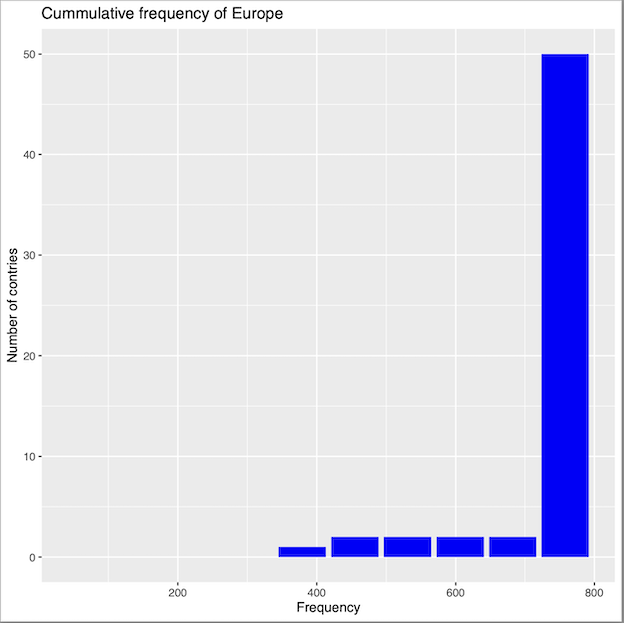
\includegraphics[scale=0.6]{images/4.1.3.png}
    \end{figure}
    \end{block}
}
\frame
{
    \frametitle{Task 4-Subtask 1}
    \begin{block}{Biểu đồ tần số tích lũy của Bắc Mỹ}
    \begin{figure}
        \centering
        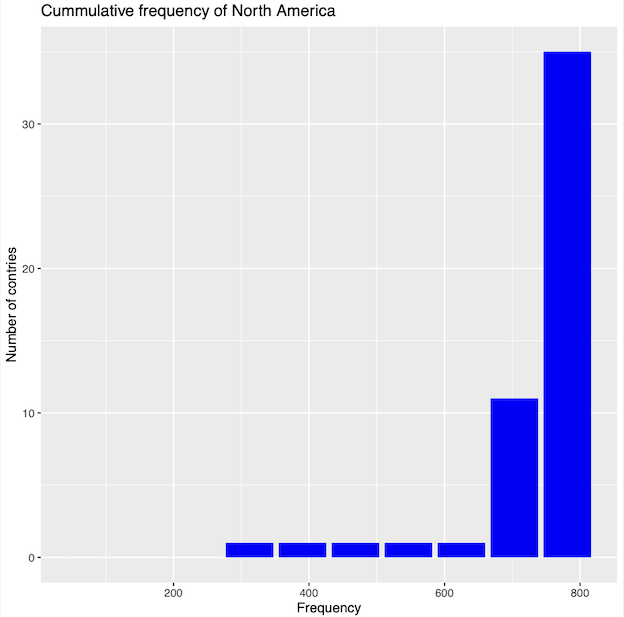
\includegraphics[scale=0.6]{images/4.1.4.png}
    \end{figure}
    \end{block}
}
{
    \frametitle{Task 4-Subtask 1}
    \begin{block}{Biểu đồ tần số tích lũy của Nam Mỹ}
    \begin{figure}
        \centering
        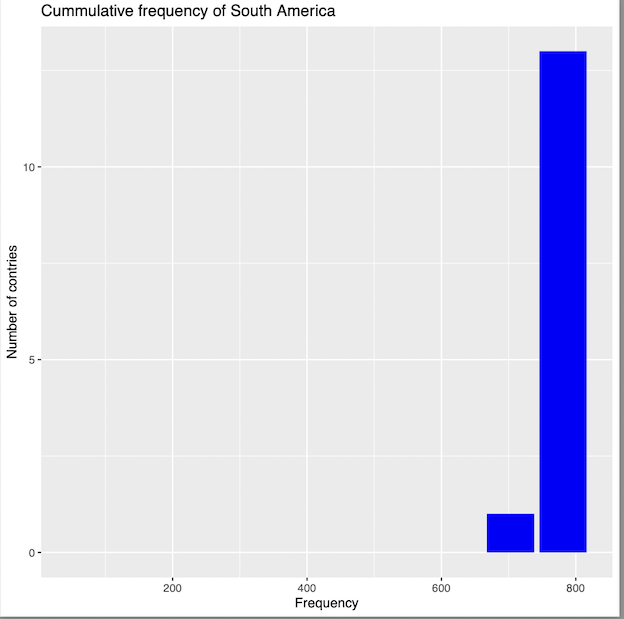
\includegraphics[scale=0.6]{images/4.1.5.png}
    \end{figure}
    \end{block}
}
{
    \frametitle{Task 4-Subtask 1}
    \begin{block}{Biểu đồ tần số tích lũy của Châu Đại Dương}
    \begin{figure}
        \centering
        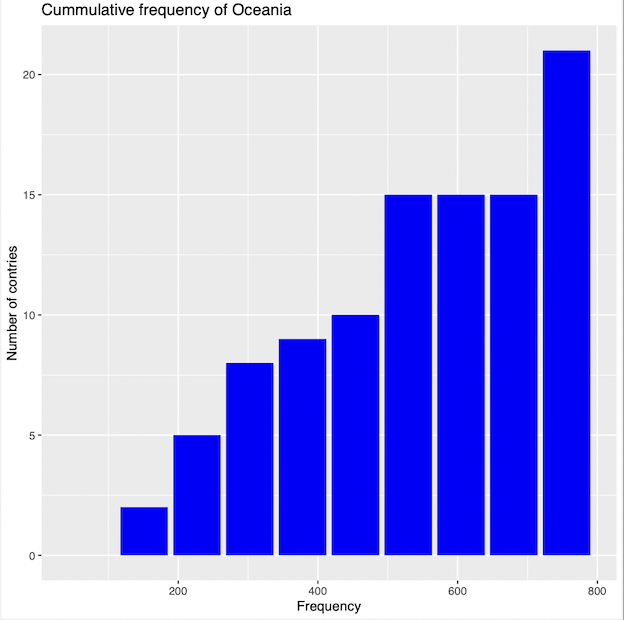
\includegraphics[scale=0.6]{images/4.1.6.png}
    \end{figure}
    \end{block}
}
\frame
{
    \frametitle{Task 4-Subtask 2}
    \begin{block}{Biểu đồ tương đối của châu Phi}
    \begin{figure}
        \centering
        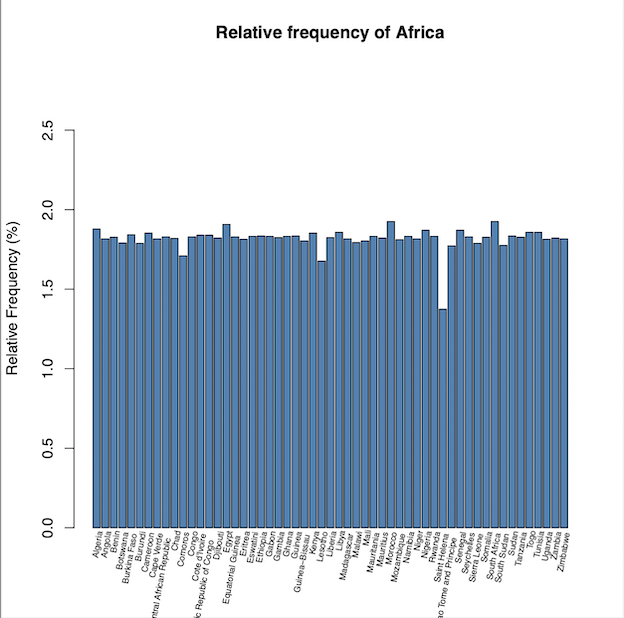
\includegraphics[scale=0.5]{images/4.2.1.png}
    \end{figure}
    \end{block}
}
\frame
{
    \frametitle{Task 4-Subtask 2}
    \begin{block}{Biểu đồ tương đối của Châu Á}
    \begin{figure}
        \centering
        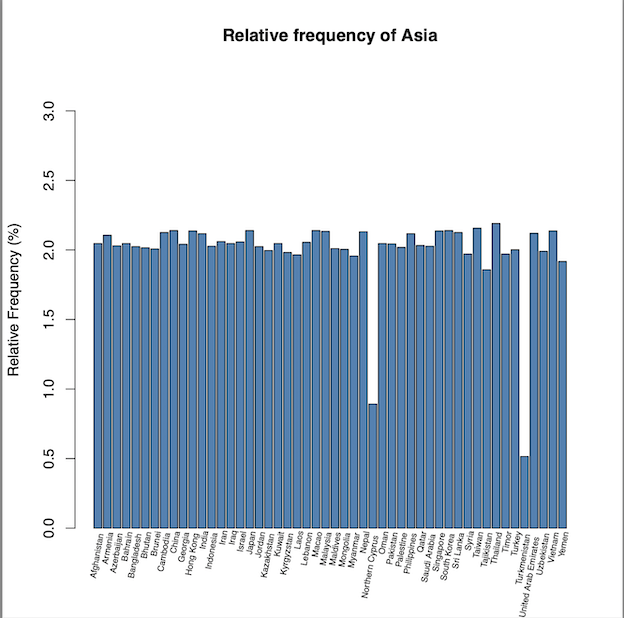
\includegraphics[scale=0.5]{images/4.2.2.png}
    \end{figure}
    \end{block}
}
\frame
{
    \frametitle{Task 4-Subtask 2}
    \begin{block}{Biểu đồ tương đối của Châu Âu}
    \begin{figure}
        \centering
        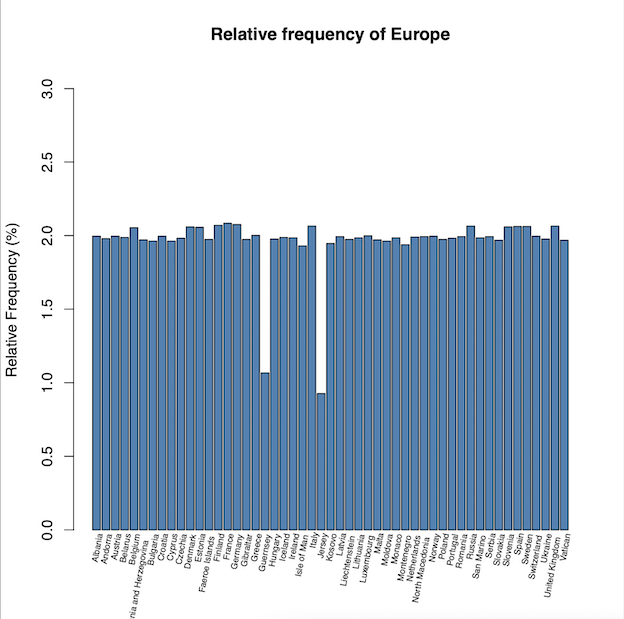
\includegraphics[scale=0.5]{images/4.2.3.png}
    \end{figure}
    \end{block}
}
\frame
{
    \frametitle{Task 4-Subtask 2}
    \begin{block}{Biểu đồ tương đối của Bắc Mỹ}
    \begin{figure}
        \centering
        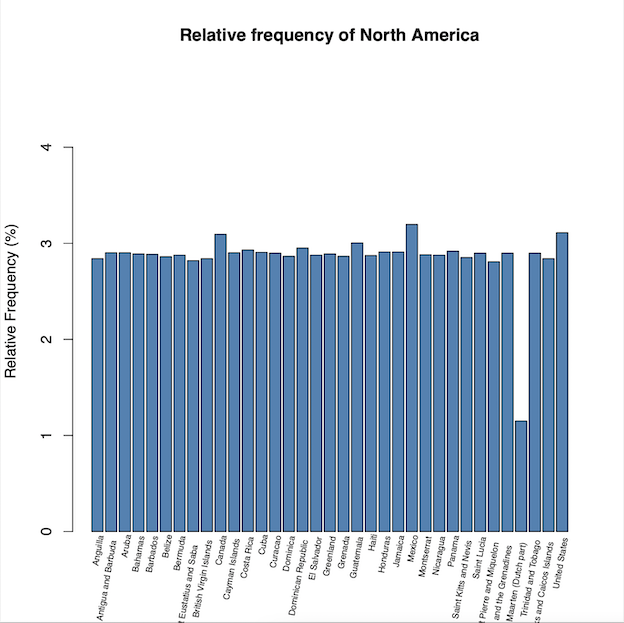
\includegraphics[scale=0.5]{images/4.2.4.png}
    \end{figure}
    \end{block}
}
\frame
{
    \frametitle{Task 4-Subtask 2}
    \begin{block}{Biểu đồ tương đối của Nam Mỹ}
    \begin{figure}
        \centering
        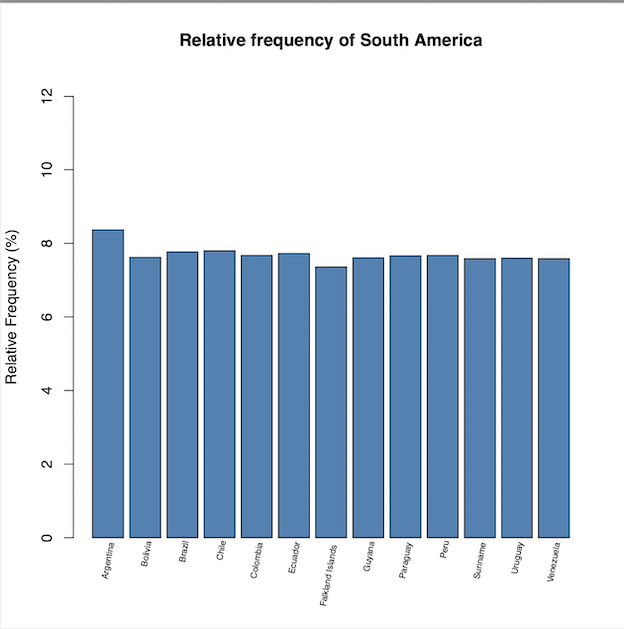
\includegraphics[scale=0.5]{images/4.2.5.png}
    \end{figure}
    \end{block}
}
\frame
{
    \frametitle{Task 4-Subtask 2}
    \begin{block}{Biểu đồ tương đối của Châu Đại Dương}
    \begin{figure}
        \centering
        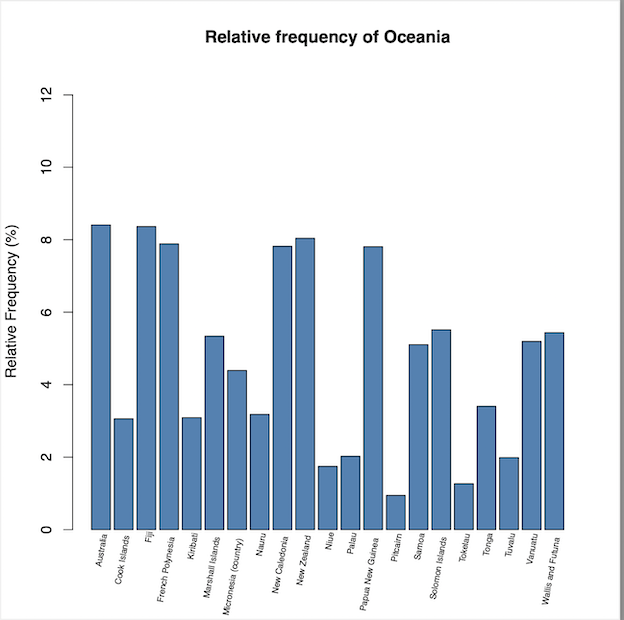
\includegraphics[scale=0.5]{images/4.2.6.png}
    \end{figure}
    \end{block}
}


\frame
{
    \frametitle{Task 4-Subtask 4}
    \begin{block}{Biểu đồ thể hiện tử vong đã báo cáo của United States trong 7 ngày cuối của năm cuối cùng}
    \begin{figure}[H]
		\centering
		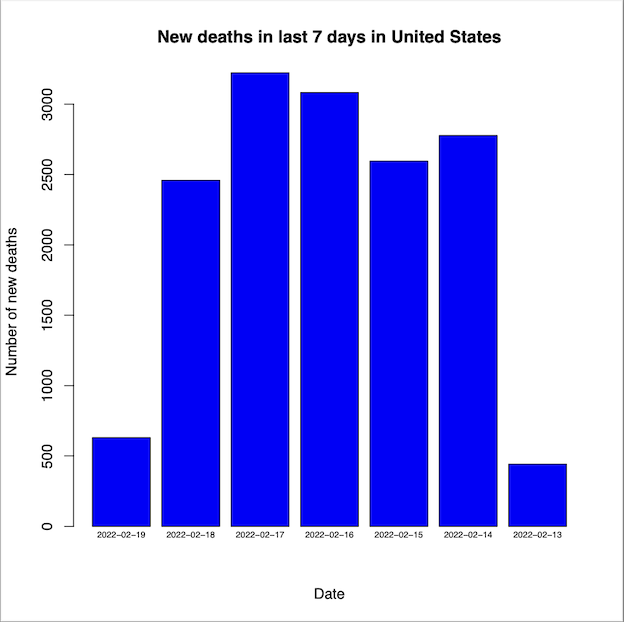
\includegraphics[scale=0.6]{images/4.3.1.png}
	\end{figure}
    \end{block}
}
\frame
{
    \frametitle{Task 4-Subtask 4}
    \begin{block}{Biểu đồ thể hiện tử vong đã báo cáo của Canada trong 7 ngày cuối của năm cuối cùng}
    \begin{figure}[H]
		\centering
		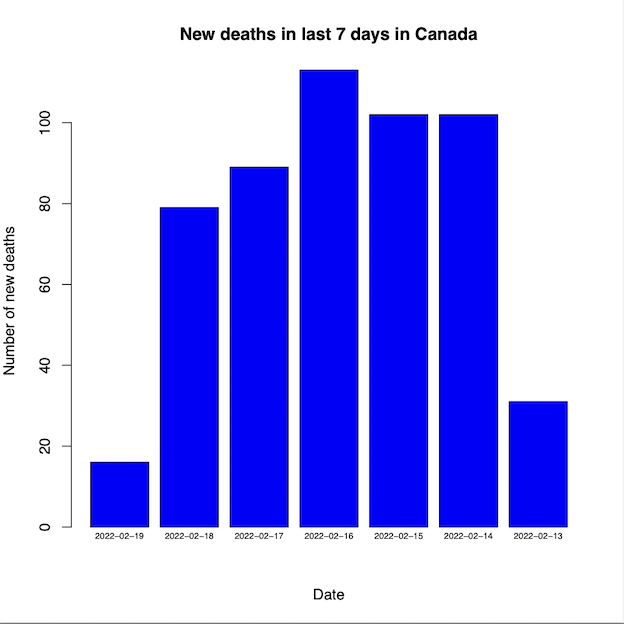
\includegraphics[scale=0.6]{images/4.3.2.png}
	\end{figure}
    \end{block}
}
\frame
{
    \frametitle{Task 4-Subtask 4}
    \begin{block}{Biểu đồ thể hiện tử vong đã báo cáo của Greenland trong 7 ngày cuối của năm cuối cùng}
    \begin{figure}[H]
		\centering
		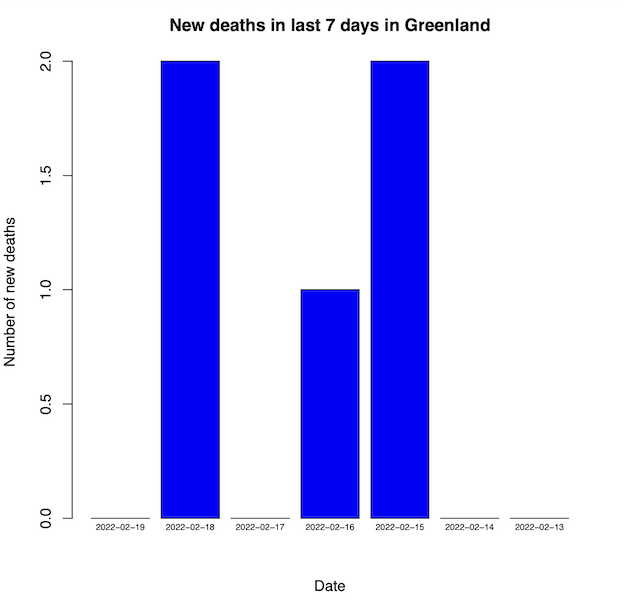
\includegraphics[scale=0.6]{images/4.3.3.png}
	\end{figure}
    \end{block}
}

\frame
{
    \frametitle{Task 4-Subtask 4}
    \begin{block}{Biểu đồ thể hiện nhiễm bệnh đã báo cáo của United States trong 7 ngày cuối của năm cuối cùng}
    \begin{figure}[H]
		\centering
		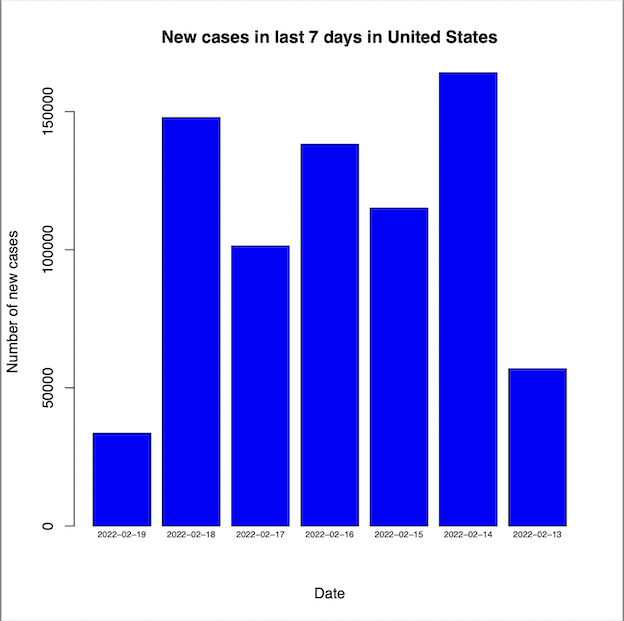
\includegraphics[scale=0.6]{images/4.4.1.png}
	\end{figure}
    \end{block}
}
{
    \frametitle{Task 4-Subtask 4}
    \begin{block}{Biểu đồ thể hiện nhiễm bệnh đã báo cáo của Canada trong 7 ngày cuối của năm cuối cùng}
    \begin{figure}[H]
		\centering
		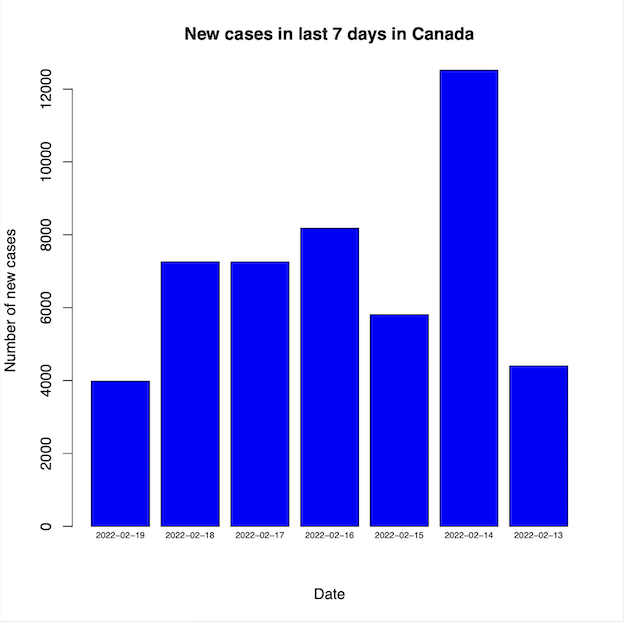
\includegraphics[scale=0.6]{images/4.4.2.png}
	\end{figure}
    \end{block}
}
{
    \frametitle{Task 4-Subtask 4}
    \begin{block}{Biểu đồ thể hiện nhiễm bệnh đã báo cáo của Greenland trong 7 ngày cuối của năm cuối cùng}
    \begin{figure}[H]
		\centering
		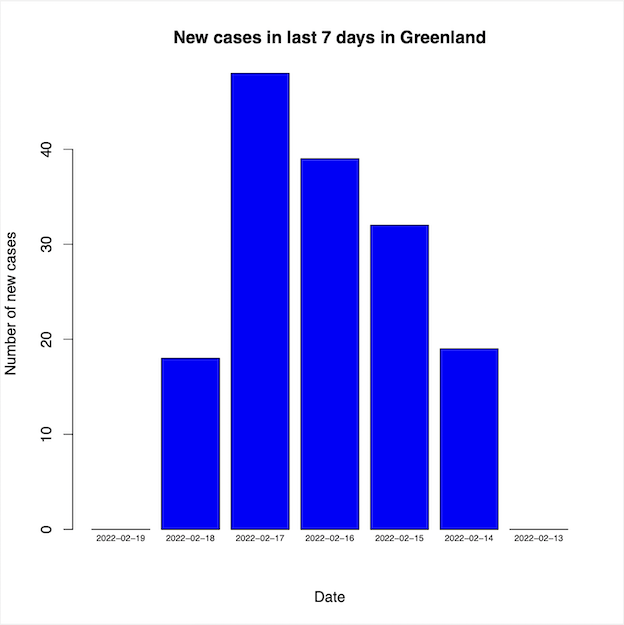
\includegraphics[scale=0.6]{images/4.4.3.png}
	\end{figure}
    \end{block}
}

\frame
{
    \frametitle{Task 4-Subtask 5}
    \begin{block}{Biểu đồ phổ đất nước xuất hiện outliers cho nhiễm bệnh}
    \begin{figure}[H]
		\centering
		\includegraphics[scale=0.6]{images/4.5.png}
	\end{figure}
    \end{block}
}
\frame
{
    \frametitle{Task 4-Subtask 5}
    \begin{block}{Biểu đồ phổ đất nước xuất hiện outliers cho tử vong}
    \begin{figure}[H]
		\centering
		\includegraphics[scale=0.6]{images/4.6.png}
	\end{figure}
    \end{block}
}


\frame
{
    \frametitle{Task 5}
    \begin{block}{Cơ sở lý thuyết}
    \begin{itemize}
        \item Số ca nhiễm của 1 ngày trong tháng bằng số ca nhiễm trong ngày hôm đó cộng với tổng số ca nhiễm của tất cả các ngày trước đó
        \item Lấy số ca nhiễm từng ngày trong tháng chia cho số ca nhiễm của ngày cuối cùng, được phần trăm số ca nhiễm tích lũy mà ngày đó đạt được so với tổng số ca nhiễm trong tháng.
        \item Các hàm dùng trong task 5: length, for, if, as.Data, data.frame, ggplot, goemline, theme, labs, is.na
    \end{itemize}
    \end{block}
}
\frame
{
    \frametitle{Task 5-Subtask 1}
    \begin{block}{Hướng làm}
        	$\indent$Đầu tiên ta lấy dữ liệu từ file owid-covid-data vào dataRaw và lọc lại các dữ liệu của các nước trong mã đề vào dataMade:
	            \begin{figure}[H]
				    \centering
				    \includegraphics[scale=0.5]{images/5.0.png}
		    	\end{figure}
	Chuyển kiểu dữ liệu của cột date từ "numberic" sang "date" và đổi tất cả giá trị N/a của cộ new\_deaths và new\_cases thành giá trị 0
	            \begin{figure}[H]
				    \centering
				    \includegraphics[scale=0.5]{images/5.0.1.png}
		    	\end{figure}
    \end{block}
}
\frame
{
    \frametitle{Task 5-Subtask 1}
    \begin{block}{Hướng làm}
        Vì 3 câu 1, 2, 3 yêu cầu vẽ biểu đồ trùng khoảng thời gian với nhau nên chỉ cần lọc dữ liệu 1 lần và sử dụng cho cả 3 câu.
	
	VD: Lọc dữ liệu số ca nhiễm bệnh và số ca tử vong ở Canada năm 2020 theo các tháng của mã đề (2, 3, 4, 6) và vẽ biểu đồ số ca nhiễm theo tháng:
	            \begin{figure}[H]
				    \centering
				    \includegraphics[scale=0.2]{images/5.0.2.png}
		    	\end{figure}
    Tương tự cho 2 nước Greenland, USA và tương tự trong 2 năm 2021, 2022.
    
    Sau khi có dữ liệu thì dùng ggpplot vẽ biểu đồ:
    
    VD: Biểu đồ số ca nhiễm theo tháng của Canada năm 2020:
                \begin{figure}[H]
				    \centering
				    \includegraphics[scale=0.2]{images/5.0.3.png}
		    	\end{figure}
    \end{block}
}
\frame
{
    \frametitle{Task 5-Subtask 1}
    \begin{block}{Biểu đồ thể hiện thu thập dữ liệu nhiễm bệnh cho từng tháng}
    \begin{figure}[H]
		\centering
	    \includegraphics[scale=0.5]{images/5.1.png}
	\end{figure}
    \end{block}
}
\frame
{
    \frametitle{Task 5-Subtask 1}
    \begin{block}{Biểu đồ thể hiện thu thập dữ liệu nhiễm bệnh cho từng tháng}
    \begin{figure}[H]
		\centering
	    \includegraphics[scale=0.5]{images/5.1.1.png}
	\end{figure}
    \end{block}
}
\frame
{
    \frametitle{Task 5-Subtask 1}
    \begin{block}{Biểu đồ thể hiện thu thập dữ liệu nhiễm bệnh cho từng tháng}
    \begin{figure}[H]
		\centering
	    \includegraphics[scale=0.5]{images/5.1.2.png}
	\end{figure}
    \end{block}
}
\frame
{
    \frametitle{Task 5-Subtask 2}
    \begin{block}{Biểu đồ thể hiện thu thập dữ liệu tử vong cho từng tháng}
    \begin{figure}[H]
		\centering
		\includegraphics[scale=0.5]{images/5.2.1.png}
	\end{figure}
    \end{block}
}
\frame
{
    \frametitle{Task 5-Subtask 2}
    \begin{block}{Biểu đồ thể hiện thu thập dữ liệu tử vong cho từng tháng}
    \begin{figure}[H]
		\centering
		\includegraphics[scale=0.5]{images/5.2.2.png}
	\end{figure}
    \end{block}
}
\frame
{
    \frametitle{Task 5-Subtask 2}
    \begin{block}{Biểu đồ thể hiện thu thập dữ liệu tử vong cho từng tháng}
    \begin{figure}[H]
		\centering
		\includegraphics[scale=0.5]{images/5.2.3.png}
	\end{figure}
    \end{block}
}
\frame
{
    \frametitle{Task 5-Subtask 3}
    \begin{block}{Biểu đồ thể hiện thu thập dữ liệu gồm nhiễm bệnh và tử vong cho từng tháng}
    \begin{figure}[H]
		\centering
		\includegraphics[scale=0.5]{images/5.3.1.png}
	\end{figure}
    \end{block}
}
\frame
{
    \frametitle{Task 5-Subtask 3}
    \begin{block}{Biểu đồ thể hiện thu thập dữ liệu gồm nhiễm bệnh và tử vong cho từng tháng}
    \begin{figure}[H]
		\centering
		\includegraphics[scale=0.5]{images/5.3.2.png}
	\end{figure}
    \end{block}
}
\frame
{
    \frametitle{Task 5-Subtask 3}
    \begin{block}{Biểu đồ thể hiện thu thập dữ liệu gồm nhiễm bệnh và tử vong cho từng tháng}
    \begin{figure}[H]
		\centering
		\includegraphics[scale=0.5]{images/5.3.3.png}
	\end{figure}
    \end{block}
}
\frame
{
    \frametitle{Task 5-Subtask 4}
    \begin{block}{Biểu đồ thể hiện thu thập dữ liệu nhiễm bệnh gồm 2 tháng cuối của năm}
    \begin{figure}[H]
		\centering
		\includegraphics[scale=0.5]{images/5.4.1.png}
	\end{figure}
    \end{block}
}
\frame
{
    \frametitle{Task 5-Subtask 4}
    \begin{block}{Biểu đồ thể hiện thu thập dữ liệu nhiễm bệnh gồm 2 tháng cuối của năm}
    \begin{figure}[H]
		\centering
		\includegraphics[scale=0.5]{images/5.4.2.png}
	\end{figure}
    \end{block}
}\frame
{
    \frametitle{Task 5-Subtask 4}
    \begin{block}{Biểu đồ thể hiện thu thập dữ liệu nhiễm bệnh gồm 2 tháng cuối của năm}
    \begin{figure}[H]
		\centering
		\includegraphics[scale=0.5]{images/5.4.3.png}
	\end{figure}
    \end{block}
}
\frame
{
    \frametitle{Task 5-Subtask 5}
    \begin{block}{Biểu đồ thể hiện thu thập dữ liệu tử vong gồm 2 tháng cuối của năm}
    \begin{figure}[H]
		\centering
		\includegraphics[scale=0.5]{images/5.5.1.png}
	\end{figure}
    \end{block}
}
\frame
{
    \frametitle{Task 5-Subtask 5}
    \begin{block}{Biểu đồ thể hiện thu thập dữ liệu tử vong gồm 2 tháng cuối của năm}
    \begin{figure}[H]
		\centering
		\includegraphics[scale=0.5]{images/5.5.2.png}
	\end{figure}
    \end{block}
}
\frame
{
    \frametitle{Task 5-Subtask 5}
    \begin{block}{Biểu đồ thể hiện thu thập dữ liệu tử vong gồm 2 tháng cuối của năm}
    \begin{figure}[H]
		\centering
		\includegraphics[scale=0.5]{images/5.5.3.png}
	\end{figure}
    \end{block}
}
\frame
{
    \frametitle{Task 5-Subtask 6}
    \begin{block}{Biểu đồ thể hiện thu thập dữ liệu gồm nhiễm bệnh và tử vong gồm 2 tháng cuối của năm}
    \begin{figure}[H]
		\centering
		\includegraphics[scale=0.5]{images/5.6.1.png}
	\end{figure}
    \end{block}
}
\frame
{
    \frametitle{Task 5-Subtask 6}
    \begin{block}{Biểu đồ thể hiện thu thập dữ liệu gồm nhiễm bệnh và tử vong gồm 2 tháng cuối của năm}
    \begin{figure}[H]
		\centering
		\includegraphics[scale=0.5]{images/5.6.2.png}
	\end{figure}
    \end{block}
}
\frame
{
    \frametitle{Task 5-Subtask 6}
    \begin{block}{Biểu đồ thể hiện thu thập dữ liệu gồm nhiễm bệnh và tử vong gồm 2 tháng cuối của năm}
    \begin{figure}[H]
		\centering
		\includegraphics[scale=0.5]{images/5.6.3.png}
	\end{figure}
    \end{block}
}
\frame
{
    \frametitle{Task 5-Subtask 7}
    \begin{block}{Hướng làm}
        $\indent$Đầu tiên ta tạo 1 vector gồm 4 số để lưu tổng số ca nhiễm của mỗi tháng
	
    VD: Tổng số ca nhiễm mỗi tháng trong năm 2020 của Canada
            \begin{figure}[H]
				\centering
				\includegraphics[scale=0.2]{images/5.0.4.png}
			\end{figure}
	Tiếp theo, ta biến đổi số ca nhiễm của từng ngày bằng số ca nhiễm của ngày hôm đó cộng với số ca nhiễm của các ngày còn lại trong tháng và lưu vào 1 vector có độ dài bằng độ dài cột new\_cases
	
    VD: Biến đổi số ca nhiễm của Canada trong năm 2020
            \begin{figure}[H]
				\centering
				\includegraphics[scale=0.2]{images/5.0.5.png}
			\end{figure}
    \end{block}
}
\frame
{
    \frametitle{Task 5-Subtask 7}
    \begin{block}{Hướng làm}
        	Biến đổi vector trên thành phần trăm tích lũy số ca nhiễm bằng cách chia cho tổng số ca nhiễm mỗi tháng đã tính
	
    VD: Biến đổi số ca nhiễm của Canada thành phần trăm tích lũy
            \begin{figure}[H]
				\centering
				\includegraphics[scale=0.2]{images/5.0.6.png}
			\end{figure}
	Cuối cùng, kết hợp vector trên với vector tháng và vẽ biểu đồ 
	
	VD: Biểu đồ phần trăm tích lũy số ca nhiễm bệnh ở Canada theo thời gian là tháng trong năm 2020
	        \begin{figure}[H]
				\centering
				\includegraphics[scale=0.2]{images/5.0.7.png}
			\end{figure}
    \end{block}
}
\frame
{
    \frametitle{Task 5-Subtask 7}
    \begin{block}{Biểu đồ thể hiện thu thập dữ liệu nhiễm bệnh tích lũy cho từng tháng}
    \begin{figure}[H]
		\centering
		\includegraphics[scale=0.5]{images/5.7.1.png}
	\end{figure}
    \end{block}
}
\frame
{
    \frametitle{Task 5-Subtask 7}
    \begin{block}{Biểu đồ thể hiện thu thập dữ liệu nhiễm bệnh tích lũy cho từng tháng}
    \begin{figure}[H]
		\centering
		\includegraphics[scale=0.5]{images/5.7.2.png}
	\end{figure}
    \end{block}
}
\frame
{
    \frametitle{Task 5-Subtask 7}
    \begin{block}{Biểu đồ thể hiện thu thập dữ liệu nhiễm bệnh tích lũy cho từng tháng}
    \begin{figure}[H]
		\centering
		\includegraphics[scale=0.5]{images/5.7.3.png}
	\end{figure}
    \end{block}
}
\frame
{
    \frametitle{Task 5-Subtask 8}
    \begin{block}{Biểu đồ thể hiện thu thập dữ liệu tử vong tích lũy cho từng tháng}
    \begin{figure}[H]
		\centering
		\includegraphics[scale=0.5]{images/5.8.1.png}
	\end{figure}
    \end{block}
}
\frame
{
    \frametitle{Task 5-Subtask 8}
    \begin{block}{Biểu đồ thể hiện thu thập dữ liệu tử vong tích lũy cho từng tháng}
    \begin{figure}[H]
		\centering
		\includegraphics[scale=0.5]{images/5.8.2.png}
	\end{figure}
    \end{block}
}
\frame
{
    \frametitle{Task 5-Subtask 8}
    \begin{block}{Biểu đồ thể hiện thu thập dữ liệu tử vong tích lũy cho từng tháng}
    \begin{figure}[H]
		\centering
		\includegraphics[scale=0.5]{images/5.8.3.png}
	\end{figure}
    \end{block}
}
\frame
{
    \frametitle{Task 6}
    \begin{block}{Cơ sở lý thuyết}
    \begin{figure}[H]
		\centering
		\includegraphics[height=7.8cm,width=7cm]{images/6.0.png}
	\end{figure}
    \end{block}
}
\frame
{
    \frametitle{Task 6}
    \begin{block}{Cơ sở lý thuyết}
    \begin{figure}[H]
		\centering
		\includegraphics[height=7.8cm,width=7cm]{images/6.0.1.png}
	\end{figure}
    \end{block}
}
\frame
{
    \frametitle{Task 6}
    \begin{block}{Cơ sở lý thuyết}
    \begin{figure}[H]
		\centering
		\includegraphics[height=7.8cm,width=7cm]{images/6.0.2.png}
	\end{figure}
    \end{block}
}
\frame
{
    \frametitle{Task 6}
    \begin{block}{Cơ sở lý thuyết}
    \begin{figure}[H]
		\centering
		\includegraphics[height=7.8cm,width=8cm]{images/6.0.3.png}
	\end{figure}
    \end{block}
}
\frame
{
    \frametitle{Task 6 - Subtask 1}
    \begin{block}{Biểu đồ thể hiện thu thập dữ liệu nhiễm bệnh cho từng tháng}
    \begin{figure}[H]
		\centering
		\includegraphics[scale=0.11]{images/6.1.1.png}
	\end{figure}
    \end{block}
}
\frame
{
    \frametitle{Task 6 - Subtask 1}
    \begin{block}{Biểu đồ thể hiện thu thập dữ liệu nhiễm bệnh cho từng tháng}
    \begin{figure}[H]
		\centering
		\includegraphics[scale=0.11]{images/6.1.2.png}
	\end{figure}
    \end{block}
}
\frame
{
    \frametitle{Task 6 - Subtask 1}
    \begin{block}{Biểu đồ thể hiện thu thập dữ liệu nhiễm bệnh cho từng tháng}
    \begin{figure}[H]
		\centering
		\includegraphics[scale=0.11]{images/6.1.3.png}
	\end{figure}
    \end{block}
}
\frame
{
    \frametitle{Task 6 - Subtask 2}
    \begin{block}{Biểu đồ thể hiện thu thập dữ liệu tử vong cho từng tháng}
    \begin{figure}[H]
		\centering
		\includegraphics[scale=0.11]{images/6.2.1.png}
	\end{figure}
    \end{block}
}
\frame
{
    \frametitle{Task 6 - Subtask 2}
    \begin{block}{Biểu đồ thể hiện thu thập dữ liệu tử vong cho từng tháng}
    \begin{figure}[H]
		\centering
		\includegraphics[scale=0.11]{images/6.2.2.png}
	\end{figure}
    \end{block}
}
\frame
{
    \frametitle{Task 6 - Subtask 2}
    \begin{block}{Biểu đồ thể hiện thu thập dữ liệu tử vong cho từng tháng}
    \begin{figure}[H]
		\centering
		\includegraphics[scale=0.11]{images/6.2.3.png}
	\end{figure}
    \end{block}
}
\frame
{
    \frametitle{Task 6 - Subtask 3}
    \begin{block}{Biểu đồ thể hiện thu thập dữ liệu gồm nhiễm bệnh và tử vong cho từng tháng}
    \begin{figure}[H]
		\centering
		\includegraphics[scale=0.105]{images/6.3.1.png}
	\end{figure}
    \end{block}
}
\frame
{
    \frametitle{Task 6 - Subtask 3}
    \begin{block}{Biểu đồ thể hiện thu thập dữ liệu gồm nhiễm bệnh và tử vong cho từng tháng}
    \begin{figure}[H]
		\centering
		\includegraphics[scale=0.105]{images/6.3.2.png}
	\end{figure}
    \end{block}
}
\frame
{
    \frametitle{Task 6 - Subtask 3}
    \begin{block}{Biểu đồ thể hiện thu thập dữ liệu gồm nhiễm bệnh và tử vong cho từng tháng}
    \begin{figure}[H]
		\centering
		\includegraphics[scale=0.105]{images/6.3.3.png}
	\end{figure}
    \end{block}
}
\frame
{
    \frametitle{Task 6 - Subtask 4}
    \begin{block}{Biểu đồ thể hiện thu thập dữ liệu nhiễm bệnh gồm 2 tháng cuối của năm}
    \begin{figure}[H]
		\centering
		\includegraphics[scale=0.105]{images/6.4.1.png}
	\end{figure}
    \end{block}
}
\frame
{
    \frametitle{Task 6 - Subtask 4}
    \begin{block}{Biểu đồ thể hiện thu thập dữ liệu nhiễm bệnh gồm 2 tháng cuối của năm}
    \begin{figure}[H]
		\centering
		\includegraphics[scale=0.105]{images/6.4.2.png}
	\end{figure}
    \end{block}
}
\frame
{
    \frametitle{Task 6 - Subtask 4}
    \begin{block}{Biểu đồ thể hiện thu thập dữ liệu nhiễm bệnh gồm 2 tháng cuối của năm}
    \begin{figure}[H]
		\centering
		\includegraphics[scale=0.105]{images/6.4.3.png}
	\end{figure}
    \end{block}
}
\frame
{
    \frametitle{Task 6 - Subtask 5}
    \begin{block}{Biểu đồ thể hiện thu thập dữ liệu tử vong gồm 2 tháng cuối của năm}
    \begin{figure}[H]
		\centering
		\includegraphics[scale=0.105]{images/6.5.1.png}
	\end{figure}
    \end{block}
}
\frame
{
    \frametitle{Task 6 - Subtask 5}
    \begin{block}{Biểu đồ thể hiện thu thập dữ liệu tử vong gồm 2 tháng cuối của năm}
    \begin{figure}[H]
		\centering
		\includegraphics[scale=0.105]{images/6.5.2.png}
	\end{figure}
    \end{block}
}
\frame
{
    \frametitle{Task 6 - Subtask 5}
    \begin{block}{Biểu đồ thể hiện thu thập dữ liệu tử vong gồm 2 tháng cuối của năm}
    \begin{figure}[H]
		\centering
		\includegraphics[scale=0.105]{images/6.5.3.png}
	\end{figure}
    \end{block}
}
\frame
{
    \frametitle{Task 6 - Subtask 6}
    \begin{block}{Biểu đồ thể hiện thu thập dữ liệu gồm nhiễm bệnh và tử vong gồm 2 tháng cuối của năm}
    \begin{figure}[H]
		\centering
		\includegraphics[scale=0.105]{images/6.6.1.png}
	\end{figure}
    \end{block}
}
\frame
{
    \frametitle{Task 6 - Subtask 6}
    \begin{block}{Biểu đồ thể hiện thu thập dữ liệu gồm nhiễm bệnh và tử vong gồm 2 tháng cuối của năm}
    \begin{figure}[H]
		\centering
		\includegraphics[scale=0.105]{images/6.6.2.png}
	\end{figure}
    \end{block}
}
\frame
{
    \frametitle{Task 6 - Subtask 6}
    \begin{block}{Biểu đồ thể hiện thu thập dữ liệu gồm nhiễm bệnh và tử vong gồm 2 tháng cuối của năm}
    \begin{figure}[H]
		\centering
		\includegraphics[scale=0.105]{images/6.6.3.png}
	\end{figure}
    \end{block}
}
\frame
{
    \frametitle{Task 6 - Subtask 7}
    \begin{block}{Biểu đồ thể hiện thu thập dữ liệu nhiễm bệnh tích lũy cho từng tháng}
    \begin{figure}[H]
		\centering
		\includegraphics[scale=0.105]{images/6.7.1.png}
	\end{figure}
    \end{block}
}
\frame
{
    \frametitle{Task 6 - Subtask 7}
    \begin{block}{Biểu đồ thể hiện thu thập dữ liệu nhiễm bệnh tích lũy cho từng tháng}
    \begin{figure}[H]
		\centering
		\includegraphics[scale=0.105]{images/6.7.2.png}
	\end{figure}
    \end{block}
}
\frame
{
    \frametitle{Task 6 - Subtask 7}
    \begin{block}{Biểu đồ thể hiện thu thập dữ liệu nhiễm bệnh tích lũy cho từng tháng}
    \begin{figure}[H]
		\centering
		\includegraphics[scale=0.105]{images/6.7.3.png}
	\end{figure}
    \end{block}
}
\frame
{
    \frametitle{Task 6 - Subtask 8}
    \begin{block}{Biểu đồ thể hiện thu thập dữ liệu tử vong tích lũy cho từng tháng}
    \begin{figure}[H]
		\centering
		\includegraphics[scale=0.11]{images/6.8.1.png}
	\end{figure}
    \end{block}
}
\frame
{
    \frametitle{Task 6 - Subtask 8}
    \begin{block}{Biểu đồ thể hiện thu thập dữ liệu tử vong tích lũy cho từng tháng}
    \begin{figure}[H]
		\centering
		\includegraphics[scale=0.11]{images/6.8.2.png}
	\end{figure}
    \end{block}
}
\frame
{
    \frametitle{Task 6 - Subtask 8}
    \begin{block}{Biểu đồ thể hiện thu thập dữ liệu tử vong tích lũy cho từng tháng}
    \begin{figure}[H]
		\centering
		\includegraphics[scale=0.11]{images/6.8.3.png}
	\end{figure}
    \end{block}
}
\frame
{
    \frametitle{Task 7}
    \begin{block}{Cơ sở lý thuyết}
    Đầu tiên ta lấy dữ liệu từ file owid-covid-data vào dataRaw và lọc lại các dữ liệu của tất cả 18 quốc gia trong đề vào dataMade:
    \begin{figure}[H]
		\centering
		\includegraphics[scale=0.6]{images/7.0.png}
	\end{figure}
    \end{block}
}
\frame
{
    \frametitle{Task 7 - Subtask 1}
    \begin{block}{Hướng làm}
    Tạo các vector ngày tháng cần thiết để lọc dữ liệu theo thời gian là tháng
	\begin{figure}[H]
		\centering
		\includegraphics[scale=0.6]{images/7.0.1.png}
	\end{figure}
    \end{block}
}
\frame
{
    \frametitle{Task 7 - Subtask 1}
    \begin{block}{Hướng làm}
    Tạo 1 vector có chiều dài là 162 để lưu dữ liệu nhiễm bệnh theo từng tháng của tất cả các quốc gia
	\begin{figure}[H]
		\centering
		\includegraphics[scale=0.6]{images/7.0.2.png}
	\end{figure}
    \end{block}
}
\frame
{
    \frametitle{Task 7 - Subtask 1}
    \begin{block}{Hướng làm}
    Chạy vòng lặp với điều kiện để lưu dữ liệu cần thiết vào vector newcases
	\begin{figure}[H]
		\centering
		\includegraphics[scale=0.55]{images/7.0.3.png}
	\end{figure}
    \end{block}
}
\frame
{
    \frametitle{Task 7 - Subtask 1}
    \begin{block}{Hướng làm}
    Kết hợp vector trên với vector tháng năm tạo thành bảng dữ liệu nhiễm bệnh theo thời gian là tháng của tất cả các nước
	\begin{figure}[H]
		\centering
		\includegraphics[scale=0.55]{images/7.0.4.png}
	\end{figure}
    \end{block}
}
\frame
{
    \frametitle{Task 7 - Subtask 1}
    \begin{block}{Hướng làm}
    Vẽ biểu đồ thể hiện thu thập dữ liệu nhiễm bệnh cho từng tháng dựa vào bảng trên
	\begin{figure}[H]
		\centering
		\includegraphics[scale=0.6]{images/7.0.5.png}
	\end{figure}
    \end{block}
}
\frame
{
    \frametitle{Task 7 - Subtask 1}
    \begin{block}{Biểu đồ thể hiện thu thập dữ liệu nhiễm bệnh theo thời gian là tháng của tất cả quốc gia}
	\begin{figure}[H]
		\centering
		\includegraphics[height=7.3cm,width=6cm]{images/7.1.png}
	\end{figure}
    \end{block}
}
\frame
{
    \frametitle{Task 7 - Subtask 2}
    \begin{block}{Biểu đồ thể hiện thu thập dữ liệu tử vong theo thời gian là tháng của tất cả quốc gia}
	\begin{figure}[H]
		\centering
		\includegraphics[height=7.3cm,width=6cm]{images/7.2.png}
	\end{figure}
    \end{block}
}
\frame
{
    \frametitle{Task 7 - Subtask 3}
    \begin{block}{Biểu đồ thể hiện thu thập dữ liệu nhiễm bệnh theo thời gian là 2 tháng cuối của năm của tất cả quốc gia}
	\begin{figure}[H]
		\centering
		\includegraphics[height=7.3cm,width=6cm]{images/7.3.png}
	\end{figure}
    \end{block}
}
\frame
{
    \frametitle{Task 7 - Subtask 4}
    \begin{block}{Biểu đồ thể hiện thu thập dữ liệu tử vong theo thời gian là 2 tháng cuối của năm của tất cả quốc gia}
	\begin{figure}[H]
		\centering
		\includegraphics[height=7.3cm,width=6cm]{images/7.4.png}
	\end{figure}
    \end{block}
}
\frame
{
    \frametitle{Task 7 - Subtask 5}
    \begin{block}{Hướng làm}
    Đầu tiên, tạo và lưu dữ liệu tích lũy nhiễm bệnh theo ngày trong 2 tháng cuối năm vào vector có độ dài 61
	\begin{figure}[H]
		\centering
		\includegraphics[height=6cm,width=9.5cm]{images/7.0.6.png}
	\end{figure}
    \end{block}
}
\frame
{
    \frametitle{Task 7 - Subtask 5}
    \begin{block}{Hướng làm}
    Tiếp theo, tạo vector có độ dài tương ứng để lưu dữ liệu nhiễm bệnh tương đối tích lũy theo thời gian là tháng bằng cách chia tất cả giá trị cho giá trị cuối cùng
	\begin{figure}[H]
		\centering
		\includegraphics[height=0.6cm,width=9.5cm]{images/7.0.7.png}
	\end{figure}
    \end{block}
}
\frame
{
    \frametitle{Task 7 - Subtask 5}
    \begin{block}{Hướng làm}
    Cuối cùng, tạo bảng dữ liệu và vẽ biểu đồ
	\begin{figure}[H]
		\centering
		\includegraphics[height=2cm,width=9.5cm]{images/7.0.8.png}
	\end{figure}
	Năm 2021 làm tương tự
    \end{block}
}
\frame
{
    \frametitle{Task 7 - Subtask 5}
    \begin{block}{Biểu đồ thể hiện thu thập dữ liệu nhiễm bệnh tương đối tích lũy theo thời gian là 2 tháng cuối của năm của tất cả quốc gia}
    \begin{figure}[H]
		\centering
		\includegraphics[height=7.3cm,width=6cm]{images/7.5.1.png}
	\end{figure}
    \end{block}
}
\frame
{
    \frametitle{Task 7 - Subtask 5}
    \begin{block}{Biểu đồ thể hiện thu thập dữ liệu nhiễm bệnh tương đối tích lũy theo thời gian là 2 tháng cuối của năm của tất cả quốc gia}
    \begin{figure}[H]
		\centering
		\includegraphics[height=7.3cm,width=6cm]{images/7.5.2.png}
	\end{figure}
    \end{block}
}
\frame
{
    \frametitle{Task 7 - Subtask 6}
    \begin{block}{Biểu đồ thể hiện thu thập dữ liệu tử vong tương đối tích lũy theo thời gian là 2 tháng cuối của năm của tất cả quốc gia}
    \begin{figure}[H]
		\centering
		\includegraphics[height=7.3cm,width=6cm]{images/7.6.1.png}
	\end{figure}
    \end{block}
}
\frame
{
    \frametitle{Task 7 - Subtask 6}
    \begin{block}{Biểu đồ thể hiện thu thập dữ liệu tử vong tương đối tích lũy theo thời gian là 2 tháng cuối của năm của tất cả quốc gia}
    \begin{figure}[H]
		\centering
		\includegraphics[height=7.3cm,width=6cm]{images/7.6.2.png}
	\end{figure}
    \end{block}
}
\frame
{
    \frametitle{Task 8}
    \begin{block}{Cơ sở lý thuyết}
    -Nghiên cứu tình trạng nhiễm bệnh và tử vong tích lũy theo thời gian là tháng tất cả các quốc gia vào tháng 2,3,4,6.\\

        *Sử dụng ngôn ngữ lập trình R để chọn lọc dữ liệu:\\

        -Lọc và xử lý dữ liệu có isocode là "OWID\_WRL", ta được các thông tin cần thiết về số ca tử vong do COVID-19 trên thế giới.\\

        *Sử dụng ngôn ngữ lập trình R để tính toán:\\

        -Bảng giá trị trung bình 7 ngày gần nhất (TB) của một dãy số A được tính như sau:\\
        \begin{itemize}
            \item TB[1]: nhận A[1]\\
            \item TB[2]: lấy giá trị trung bình của A[1], A[2]\\
            \item TB[3]: lấy giá trị trung bình của A[1], A[2], A[3]\\
            \item .\\
            \item .\\
            \item TB[7]: lấy giá trị trung bình của A[1], A[2], ..., A[7]\\
            \item TB[i] (i>7): lấy giá trị trung bình của A[i-6], A[i-5],..., A[i]\\
        \end{itemize}
    \end{block}
}
\frame
{
    \frametitle{Task 8}
    \begin{block}{Cơ sở lý thuyết}
    -Từng bước khởi gán các giá trị tổng số ca nhiễm, tử vong theo tháng, sau đó tính trung bình 7 ngày gần nhất của từng ngày và đồng thời tạo bảng giá trị theo từng tháng, từng năm và từng nhóm câu hỏi của đề bài\\

        *Sử dụng ngôn ngữ R để vẽ biểu đồ cho từng nhóm câu hỏi*\\

        -Đầu tiên, tạo các biến cần thiết:\\
        ggplot(NULL,aes(<các ngày>,<số ca mới>)): khởi tạo hệ trục Oxy với các miền giá trị tương ứng Ox,Oy\\
        geomline(data=<new>,col="<colour>"): vẽ đường biểu diễn các ca mới (new) trong tháng, có màu là (colour)\\
        labs(title="<tên biểu đồ>",x="<tên trục Ox>,y="<tên trục Oy>"): thêm nhãn cho biểu đồ\\
        
        -Tiếp theo, kết hợp các biến vào một để tạo biểu đồ\\
        graphcases<tháng hiện tại><-ggplot()+geomline()+labs(): tạo biểu đồ theo tháng đang tính toán( 4 tháng tất cả)\\
    \end{block}
}
\frame
{
    \frametitle{Task 8}
    \begin{block}{Cơ sở lý thuyết}
    -Cuối cùng, lưu các biểu đồ vừa tạo vào một file lưu trữ\\
        -Ví dụ:\\
        \begin{itemize}
            \item ggsave(filename="task8subtask1case2020.pdf",\\
            \item plot=ggarrange(graphcasesthangHai, graphcasesthangBa,graphcasesthangTu,graphcasesthangSau, nrow=4, ncol=1, common.legend=TRUE),\\
            \item scale=1,\\
            \item width=10,\\
            \item height=25,\\
            \item units=c("in"),\\
            \item dpi=300)\\
        \end{itemize}
        --->tạo file có tên "task8subtask1case2020.pdf" lưu số ca mới trong năm 2020 theo yêu cầu tiểu câu hỏi 1 với 4 biểu đồ riêng biệt của 4 tháng 2,3,4,6 xếp dọc 4 hàng 1 cột, tỉ lệ phóng đại 1.0, chiều rộng 10 inch, chiều cao 25 inch\\
        
        (Có sử dụng thêm các lệnh trên biểu đồ để trang trí, hiệu chỉnh)
    \end{block}
}
\frame
{
    \frametitle{Task 8 - Subtask 1}
    \begin{block}{Biểu đồ thể hiện thu thập dữ liệu nhiễm bệnh theo thời gian là tháng của tất cả quốc gia theo trung bình 7 ngày gần nhất}
    \begin{figure}[H]
			\centering
			\includegraphics[height=7.5cm,width=4.2cm]{images/8.1.1.png}
	\end{figure}
    \end{block}
}
\frame
{
    \frametitle{Task 8 - Subtask 1}
    \begin{block}{Biểu đồ thể hiện thu thập dữ liệu nhiễm bệnh theo thời gian là tháng của tất cả quốc gia theo trung bình 7 ngày gần nhất}
    \begin{figure}[H]
			\centering
			\includegraphics[height=7.5cm,width=4.2cm]{images/8.1.2.png}
	\end{figure}
    \end{block}
}
\frame
{
    \frametitle{Task 8 - Subtask 1}
    \begin{block}{Biểu đồ thể hiện thu thập dữ liệu nhiễm bệnh theo thời gian là tháng của tất cả quốc gia theo trung bình 7 ngày gần nhất}
    \begin{figure}[H]
			\centering
			\includegraphics[scale=0.1]{images/8.1.3.png}
	\end{figure}
    \end{block}
}
\frame
{
    \frametitle{Task 8 - Subtask 2}
    \begin{block}{Biểu đồ thể hiện thu thập dữ liệu tử vong theo thời gian là tháng của tất cả quốc gia theo trung bình 7 ngày gần nhất}
    \begin{figure}[H]
			\centering
			\includegraphics[height=7.5cm,width=4.2cm]{images/8.2.1.png}
	\end{figure}
    \end{block}
}
\frame
{
    \frametitle{Task 8 - Subtask 2}
    \begin{block}{Biểu đồ thể hiện thu thập dữ liệu tử vong theo thời gian là tháng của tất cả quốc gia theo trung bình 7 ngày gần nhất}
    \begin{figure}[H]
			\centering
			\includegraphics[height=7.5cm,width=4.2cm]{images/8.2.2.png}
	\end{figure}
    \end{block}
}
\frame
{
    \frametitle{Task 8 - Subtask 2}
    \begin{block}{Biểu đồ thể hiện thu thập dữ liệu tử vong theo thời gian là tháng của tất cả quốc gia theo trung bình 7 ngày gần nhất}
    \begin{figure}[H]
			\centering
			\includegraphics[scale=0.1]{images/8.2.3.png}
	\end{figure}
    \end{block}
}
\frame
{
    \frametitle{Task 8 - Subtask 3}
    \begin{block}{Biểu đồ thể hiện thu thập dữ liệu nhiễm bệnh theo thời gian là 2 tháng của năm của tất cả quốc giaị theo trung bình 7 ngày gần nhất}
    \begin{figure}[H]
			\centering
			\includegraphics[height=7cm,width=4.2cm]{images/8.3.1.png}
	\end{figure}
    \end{block}
}
\frame
{
    \frametitle{Task 8 - Subtask 3}
    \begin{block}{Biểu đồ thể hiện thu thập dữ liệu nhiễm bệnh theo thời gian là 2 tháng của năm của tất cả quốc giaị theo trung bình 7 ngày gần nhất}
    \begin{figure}[H]
			\centering
			\includegraphics[height=7cm,width=4.2cm]{images/8.3.2.png}
	\end{figure}
    \end{block}
}
\frame
{
    \frametitle{Task 8 - Subtask 3}
    \begin{block}{Biểu đồ thể hiện thu thập dữ liệu nhiễm bệnh theo thời gian là 2 tháng của năm của tất cả quốc giaị theo trung bình 7 ngày gần nhất}
    \begin{figure}[H]
			\centering
			\includegraphics[scale=0.1]{images/8.3.3.png}
	\end{figure}
    \end{block}
}
\frame
{
    \frametitle{Task 8 - Subtask 4}
    \begin{block}{Biểu đồ thể hiện thu thập dữ liệu tử vong theo thời gian là 2 tháng của năm của tất cả quốc gia theo trung bình 7 ngày gần nhất}
    \begin{figure}[H]
			\centering
			\includegraphics[height=7.5cm,width=4.2cm]{images/8.4.1.png}
	\end{figure}
    \end{block}
}
\frame
{
    \frametitle{Task 8 - Subtask 4}
    \begin{block}{Biểu đồ thể hiện thu thập dữ liệu tử vong theo thời gian là 2 tháng của năm của tất cả quốc gia theo trung bình 7 ngày gần nhất}
    \begin{figure}[H]
			\centering
			\includegraphics[height=7.5cm,width=4.2cm]{images/8.4.2.png}
	\end{figure}
    \end{block}
}
\frame
{
    \frametitle{Task 8 - Subtask 4}
    \begin{block}{Biểu đồ thể hiện thu thập dữ liệu tử vong theo thời gian là 2 tháng của năm của tất cả quốc gia theo trung bình 7 ngày gần nhất}
    \begin{figure}[H]
			\centering
			\includegraphics[scale=0.1]{images/8.4.3.png}
	\end{figure}
    \end{block}
}
\frame
{
    \frametitle{Task 8 - Subtask 5}
    \begin{block}{Biểu đồ thể hiện thu thập dữ liệu nhiễm bệnh tích lũy theo thời gian là 2 tháng của năm của tất cả quốc gia theo trung bình 7 ngày gần nhất}
    \begin{figure}[H]
			\centering
			\includegraphics[height=7cm,width=4.2cm]{images/8.5.1.png}
	\end{figure}
    \end{block}
}
\frame
{
    \frametitle{Task 8 - Subtask 5}
    \begin{block}{Biểu đồ thể hiện thu thập dữ liệu nhiễm bệnh tích lũy theo thời gian là 2 tháng của năm của tất cả quốc giaị theo trung bình 7 ngày gần nhất}
    \begin{figure}[H]
			\centering
			\includegraphics[height=7cm,width=4.2cm]{images/8.5.2.png}
	\end{figure}
    \end{block}
}
\frame
{
    \frametitle{Task 8 - Subtask 5}
    \begin{block}{Biểu đồ thể hiện thu thập dữ liệu nhiễm bệnh tích lũy theo thời gian là 2 tháng của năm của tất cả quốc giaị theo trung bình 7 ngày gần nhất}
    \begin{figure}[H]
			\centering
			\includegraphics[scale=0.1]{images/8.5.3.png}
	\end{figure}
    \end{block}
}
\frame
{
    \frametitle{Task 8 - Subtask 6}
    \begin{block}{Biểu đồ thể hiện thu thập dữ liệu tử vong tích lũy theo thời gian là 2 tháng của năm của tất cả quốc gia theo trung bình 7 ngày gần nhất}
    \begin{figure}[H]
			\centering
			\includegraphics[height=7cm,width=4.2cm]{images/8.6.1.png}
	\end{figure}
    \end{block}
}
\frame
{
    \frametitle{Task 8 - Subtask 6}
    \begin{block}{Biểu đồ thể hiện thu thập dữ liệu tử vong tích lũy theo thời gian là 2 tháng của năm của tất cả quốc gia theo trung bình 7 ngày gần nhất}
    \begin{figure}[H]
			\centering
			\includegraphics[height=7cm,width=4.2cm]{images/8.6.2.png}
	\end{figure}
    \end{block}
}
\frame
{
    \frametitle{Task 8 - Subtask 6}
    \begin{block}{Biểu đồ thể hiện thu thập dữ liệu tử vong tích lũy theo thời gian là 2 tháng của năm của tất cả quốc gia theo trung bình 7 ngày gần nhất}
    \begin{figure}[H]
			\centering
			\includegraphics[scale=0.1]{images/8.6.3.png}
	\end{figure}
    \end{block}
}
\frame
{
    \frametitle{Task 9}
    \begin{block}{Cơ sở lý thuyết}
    -----Correlation Coefficient là gì?-----\\
		\begin{itemize}
		    \small\item Hệ số tương quan là một thước đo thống kê về độ mạnh yếu của mối quan hệ giữa các chuyển động tương đối của hai biến, các giá trị này nằm trong khoảng từ -1,0 đến 1,0. Một số được tính toán lớn hơn 1,0 hoặc nhỏ hơn -1,0 có nghĩa là đã xảy ra lỗi trong phép đo tương quan. Tương quan -1,0 cho thấy mối tương quan âm tuyệt đối, trong khi mức tương quan 1,0 cho thấy mối tương quan dương tuyệt đối. Tương quan 0,0 cho thấy không có mối quan hệ tuyến tính giữa chuyển động của hai biến.\\
		
		    \small\item Có một loại hệ số tương quan, nhưng phổ biến nhất là hệ số tương quan Pearson (R), hệ số này chỉ ra độ mạnh và hướng của mối quan hệ tuyến tính giữa hai biến. Đây cũng là hệ số sẽ được sử dụng để tính toán trong phần trình bày này.\\
		
		    \small\item Giá trị chính xác bằng 1,0 nghĩa là có một mối quan hệ dương tuyệt đối giữa hai biến. Đối với một biến số tăng dương thì biến số thứ hai cũng tăng dương.Giá trị chính xác bằng -1,0 nghĩa là có một mối quan hệ âm tuyệt đối giữa hai biến. Điểu này cho thấy các biến chuyển động ngược chiểu nhau. Đối với một biến số tăng dương thì biến số thứ hai sẽ giảm xuống. Nếu mối tương quan giữa hai biến là 0 thì không có mối quan hệ tuyến tính giữa chúng.\\
		\end{itemize}
    \end{block}
}
\frame
{
    \frametitle{Task 9}
    \begin{block}{Cơ sở lý thuyết}
	\begin{itemize}
	    \item Độ mạnh của mối quan hệ thay đổi theo mức độ dựa trên giá trị của hệ số tương quan. Ví dụ, giá trị 0,2 cho thấy có mối tương quan dương giữa hai biến. Các nhà phân tích trong một số lĩnh vực nghiên cứu không coi các mối tương quan là quan trọng cho đến khi giá trị vượt qua ít nhất 0,8. Tuy nhiên, hệ số tương quan có giá trị tuyệt đối từ 0,9 trở lên sẽ thể hiện một mối quan hệ rất chặt chẽ.\\
	\end{itemize}
	- Trong bài báo cáo này, một mối quan hệ giữa hai biến được coi là:\\
	\begin{itemize}
	    \item Mạnh (Strong) nếu trị tuyệt đối hệ số tương quan giữa chúng lớn hơn 0,7,\\
		\item Trung bình (Moderate) nếu trị tuyệt đối hệ số tương quan giữa chúng lớn hơn 0,5 và bé hơn bằng 0,7,\\
		\item Yếu (Weak) nếu trị tuyệt đối hệ số tương quan giữa chúng lớn hơn 0,3 và bé hơn bằng 0,5,\\
		\item Rất yếu(Very Weak) nếu trị tuyệt đối hệ số tương quan giữa chúng bé hơn bằng 0,3.\\
	\end{itemize}
    \end{block}
}
\frame
{
    \frametitle{Task 9}
    \begin{block}{Cơ sở lý thuyết}
	- Nghiên cứu tình trạng nhiễm bệnh và tử vong tích lũy theo thời gian là tháng của 3 nước theo MADE vào 4 tháng 2,3,4,6\\
		
	- Lọc và xử lý dữ liệu có isocode là CAN,GRL,USA ta được các thông tin cần thiết về số ca mắc mới và số ca tử vong do COVID19 tại các nước Canada, Greenland và Hoa Kỳ.\\
		
	- Sử dụng ngôn ngữ lập trình R để tính toán:\\
	Từng bước khởi gán các giá trị tống số ca nhiễm, ca tử vong theo tháng sau đó tính tổng  tích lũy từng ngày, đông thời lập bảng tỉ lệ phần trăm trên tổng số ca.\\
	Sử dụng hàm cor(x,y,"pearson") để tính Pearson coefficient correlation giữa 2 biến, sau đó kết hợp kết quả với nhận xét về độ mạnh của mối tương quan đưa vào biểu đồ của subtask1\\
    \end{block}
}
\frame
{
    \frametitle{Task 9}
    \begin{block}{Cơ sở lý thuyết}
	Sử dụng các lệnh của ngôn ngữ R để vẽ biểu đồ:\\
	- Đầu tiên, tạo các biến cần thiết\\
	+ ggplot(NULL,aes(<các ngày>, <số ca mới>)): khởi tạo hệ trục Oxy với các miền giá trị tương ứng Ox,Oy\\
	+ geomarea(data=<new>, col="<colour>"): vẽ miền biểu diễn các ca mới (new) trong tháng, có màu là (colour)\\
	+ labs(title="<tên biểu đồ>",x="<tên trục Ox>",y="<tên trục Oy>"): thêm nhãn cho biểu đồ\\
	+annotate(geom="<kiểu chú thích>",x=<tọa độ x>, y=<tọa độ y>,...): thêm chú thích cho biểu đồ\\
		
	- Tiếp theo, kết hợp các biến vào một để tạo biểu đồ\\
	graphcases<tháng hiện tại> <- ggplot()+geomarea()+labs()+annotate(): tạo biểu đồ theo tháng đang tính toán (4 tháng tất cả)\\
		
	- Cuối cùng, lưu các biểu đồ vừa tạo vào một file lưu trữ\\
    \end{block}
}
\frame
{
    \frametitle{Task 9}
    \begin{block}{Cơ sở lý thuyết}
	Ví dụ:\\
	\begin{itemize}
	    \item ggsave(filename="task9subtask1Canadanews2020.pdf",\\
		\item plot=ggarrange(graphcasesthangHai, graphcasesthangBa,graphcasesthangTu,graphcasesthangSau, nrow=4, ncol=1, common.legend=TRUE),\\
        \item scale=1,\\
        \item width=10,\\
        \item height=25,\\
        \item units=c("in"),\\
        \item dpi=300)\\
	\end{itemize}
    --->tạo file có tên "task9subtask1Canadanews2020.pdf" lưu số ca mới trong năm 2020 theo yêu cầu tiểu câu hỏi 1 với 4 biểu đồ riêng biệt của 4 tháng 2,3,4,6 xếp dọc 4 hàng 1 cột, tỉ lệ phóng đại 1.0, chiều rộng 10 inch, chiều cao 25 inch\\
        
    (Có sử dụng thêm các lệnh trên biểu đồ để trang trí, hiệu chỉnh)
    \end{block}
}
\frame
{
    \frametitle{Task 9}
    \begin{block}{Kết quả}
	\begin{figure}[H]
		\centering
		\includegraphics[height=7.7cm,width=4.2cm]{images/9.1.png}
	\end{figure}
    \end{block}
}
\frame
{
    \frametitle{Task 9}
    \begin{block}{Kết quả}
	\begin{figure}[H]
		\centering
		\includegraphics[height=7.7cm,width=4.2cm]{images/9.2.png}
	\end{figure}
    \end{block}
}
\frame
{
    \frametitle{Task 9}
    \begin{block}{Kết quả}
	\begin{figure}[H]
		\centering
		\includegraphics[height=7.7cm,width=4.2cm]{images/9.3.png}
	\end{figure}
    \end{block}
}
\frame
{
    \frametitle{Task 9}
    \begin{block}{Kết quả}
	\begin{figure}[H]
		\centering
		\includegraphics[height=7.7cm,width=4.2cm]{images/9.4.png}
	\end{figure}
    \end{block}
}
\frame
{
    \frametitle{Task 9}
    \begin{block}{Kết quả}
	\begin{figure}[H]
		\centering
		\includegraphics[height=7.7cm,width=4.2cm]{images/9.5.png}
	\end{figure}
    \end{block}
}
\frame
{
    \frametitle{Task 9}
    \begin{block}{Kết quả}
	\begin{figure}[H]
		\centering
		\includegraphics[height=7.7cm,width=4.2cm]{images/9.6.png}
	\end{figure}
    \end{block}
}
\frame
{
    \frametitle{Task 10 - Subtask 2}
    \begin{block}{Tình trạng tử vong của các quốc gia trong 7 ngày cuối của năm cuối cùng (2022)}
	\begin{figure}[H]
        \centering
        \includegraphics[scale=0.3]{images/10.2.png}
    \end{figure}
    \end{block}
}
\frame
{
    \frametitle{Task 10 - Subtask 2}
    \begin{block}{So sánh \& Nhận xét}
	-  Trong 7 ngày cuối trong số liệu của năm cuối cùng (từ 13/02 -19/02 năm 2022):\\
    \begin{itemize}
        \item Greenland khá may mắn vì gần như không có một ca tử vong nào, cho thấy nước này đảm bảo được sự an toàn trước đại dịch.\\
        \item Bên cạnh đó, Canada lại có số người chết mỗi ngày còn khá nhiều (dao động trong vài chục ca).\\
        \item Tuy vậy, người dân Hoa Kỳ vẫn chịu nhiều sự đau thương nhất, khi mà có đến 5 trên 7 ngày số người chết lên tới 4 chữ số.\\
        \end{itemize}
    -> Những điều này chứng tỏ những ảnh hưởng nặng nề mà đại dịch này để lại cho con người, những con virut mang lại hậu quả sức khỏe hết sức nguy hiểm không thể chủ quan.\\
   \end{block}
}
\frame
{
    \frametitle{Task 10 - Subtask 4}
    \begin{block}{Cơ sở lý thuyết \& Kết quả}
    - Lấy k làm mốc để xác định khoảng thời gian bùng phát.\\
    - Với k là khi số ca nhiễm bệnh tăng đột biến trên khoảng 200 phần trăm so với 20 ngày trước, số ca nhiễm bệnh phải lớn hơn 50000 thì ta sẽ coi đó là lúc bùng phát bệnh dịch.\\
    - Từ đó, sử dụng ngôn ngữ lập trình R để chỉ ra các thời điểm bắt đầu bùng phát.\\
	\begin{figure}[H]
        \centering
        \includegraphics[scale=0.9]{images/10.4.png}
    \end{figure}
    \end{block}
}
\frame
{
    \frametitle{Task 10 - Subtask 6}
    \begin{block}{Khoảng thời gian bùng phát nhiễm bệnh lớn nhất giữa các quốc gia có chồng lên nhau không, Cho biết khoảng thời gian giao nhau đó?}
    - Các mốc bùng phát bệnh dịch của các quốc gia là:\\
        \begin{itemize}
            \item CANADA\\
            \item 2021-12-20\\
            \item GREENLAND\\
            \item NULL\\
            \item USA\\
            \item 2021-12-28\\
        \end{itemize}
    - Dễ dàng nhận thấy 2 nước Canada và Hoa Kỳ có cùng khoảng thời gian bắt đầu bùng phát bệnh dịch vào cuối năm ngoái (2021)\\
    - Đây cũng là thời điểm 2 nước này có kì nghỉ lễ đặc biệt nhất trong năm (Lễ Giáng Sinh và chuẩn bị qua năm mới).\\
    - Do đó, từ tháng 12 năm 2021 đến tháng 1 năm 2022, số ca nhiễm bệnh đã tăng không kiểm soát, với số ca nhiễm cao nhất trong 1 ngày đã tăng gấp 10 lần so với trước khi dịch bệnh bùng nổ.
    \end{block}
}
\section{Tổng kết}
\frame
{
    \frametitle{Tổng kết}
    \begin{block}{Tóm lại}
        $\indent$Phân tích dữ liệu về dịch bệnh Covid có ý nghĩa quan trọng trong việc đánh giá mức độ nghiêm trọng của đại dịch trên toàn thế giới. Ngoài ra, những dữ liệu riêng của từng châu lục, hay từng quốc gia giúp ta dễ dàng xác định được những khu vực có dịch bệnh bùng nổ, hay những nơi có dấu hiệu xuất hiện của dịch bệnh để tìm ra những biện pháp xử lý, phòng tránh phù hợp. Những kết quả ta phân tích được trong quá khứ có ý nghĩa thực tế trong việc dự đoán những con số sẽ xuất hiện trong tương lai. Qua bài tập lớn này, ngoài việc tiếp xúc và rèn luyện với ngôn ngữ mới là R và Latex, ta còn được nâng cao kỹ năng phân tích số liệu cũng như biểu diễn các số liệu thống kê một cách dễ hiểu cho người xem.
    \end{block}
}

%%%%%%%%%%%%%%%%%%%%%%%%%%%%%%%%%%%%%%%%%%%%%%%%%%%%%%%%%%%%%%%%%%%%%
%%%%%%%%%%%%%%%%%%%%%%%%%%%%%%%%%%%%%%%%%%%%%%%%%%%%%%%%%%%%%%%%%%%%%

\end{document}